\documentclass[11pt,letterpaper]{article}
\usepackage[T1]{fontenc}
\usepackage[utf8]{inputenc}
\usepackage{lmodern}
\usepackage[margin=1in,headheight=15pt]{geometry}
\usepackage{amsmath,amssymb,amsthm,mathtools}
\usepackage{microtype,booktabs,longtable,tabularx,array,enumitem}
\usepackage{tocloft}
\setlength{\cftbeforesecskip}{4pt}
\setlength{\cftbeforetoctitleskip}{0pt}
\setlength{\cftaftertoctitleskip}{12pt}
\usepackage{xcolor,fancyhdr,needspace,listings}
\usepackage{tikz}
\usetikzlibrary{arrows.meta,positioning}
\definecolor{Ink}{HTML}{213847}
\definecolor{Accent}{HTML}{236578}
\definecolor{Light}{HTML}{F0F4F6}
\usepackage[colorlinks=true,linkcolor=Ink,citecolor=Accent,urlcolor=Accent]{hyperref}
\usepackage{xurl}
\usepackage[nameinlink,noabbrev]{cleveref}
\hypersetup{pdftitle={Finite Certificates for Surcomplex Wick Summability},
 pdfauthor={Research manuscript prepared with AI assistance},
 pdfsubject={Hahn summability, finite valuation certificates, connected diagrams}}
\pagestyle{fancy}\fancyhf{}
\fancyhead[L]{\small Surcomplex Wick summability}
\fancyhead[R]{\small\thepage}
\renewcommand{\headrulewidth}{0.3pt}
\setlength{\parskip}{0.28em}
\setlength{\emergencystretch}{2.5em}
\widowpenalty=10000\clubpenalty=10000
\setlist{itemsep=0.2em,topsep=0.35em}
\setcounter{tocdepth}{2}
\numberwithin{equation}{section}
\newtheorem{theorem}{Theorem}[section]
\newtheorem{lemma}[theorem]{Lemma}
\newtheorem{proposition}[theorem]{Proposition}
\newtheorem{corollary}[theorem]{Corollary}
\theoremstyle{definition}
\newtheorem{definition}[theorem]{Definition}
\newtheorem{example}[theorem]{Example}
\newtheorem{convention}[theorem]{Convention}
\theoremstyle{remark}
\newtheorem{remark}[theorem]{Remark}
\crefname{definition}{definition}{definitions}
\Crefname{definition}{Definition}{Definitions}
\crefname{lemma}{lemma}{lemmas}
\Crefname{lemma}{Lemma}{Lemmas}
\crefname{proposition}{proposition}{propositions}
\Crefname{proposition}{Proposition}{Propositions}
\crefname{corollary}{corollary}{corollaries}
\Crefname{corollary}{Corollary}{Corollaries}
\crefname{theorem}{theorem}{theorems}
\Crefname{theorem}{Theorem}{Theorems}
\crefname{example}{example}{examples}
\Crefname{example}{Example}{Examples}
\newcommand{\No}{\mathbf{No}}
\newcommand{\SC}{\mathbf{No}[i]}
\newcommand{\R}{\mathbb R}
\newcommand{\C}{\mathbb C}
\newcommand{\Q}{\mathbb Q}
\newcommand{\N}{\mathbb N}
\newcommand{\Z}{\mathbb Z}
\newcommand{\K}{\mathbb K}
\newcommand{\KR}{\mathbb K_{\R}}
\newcommand{\EE}{\mathsf E}
\newcommand{\cZ}{\mathcal Z}
\newcommand{\cH}{\mathcal H}
\newcommand{\cP}{\mathcal P}
\newcommand{\ve}{\mathbf e}
\newcommand{\abs}[1]{\lvert#1\rvert}
\newcommand{\supp}{\operatorname{supp}}
\newcommand{\val}{\operatorname v}
\newcommand{\rank}{\operatorname{rank}}
\newcommand{\diag}{\operatorname{diag}}
\newcommand{\st}{\operatorname{st}}
\newcommand{\Commit}{\nolinkurl{4cf691c7d951e037739d32d9f5c387dcce724f3c}}
\newcommand{\Repo}{\texttt{VladimirReshetnikov/Surreal}}
\newcolumntype{Y}{>{\raggedright\arraybackslash}X}
\lstset{basicstyle=\small\ttfamily,breaklines=true,columns=fullflexible,
 frame=single,rulecolor=\color{black!20},showstringspaces=false}

\begin{document}
\hypersetup{pageanchor=false}
\begin{titlepage}
\centering
\vspace*{0.4in}
{\large\scshape Research in surreal and surcomplex analysis\par}
\vspace{0.45in}
{\LARGE\bfseries\color{Ink} Finite Certificates for\\[0.2em]
Surcomplex Wick Summability\par}
\vspace{0.25in}
{\large Valuation balancing, connected obstructions,\\[0.15em]
and multiscale Gaussian perturbations\par}
\vspace{0.35in}
{\large September 22, 2026\par}
\vspace{0.3in}
\begin{minipage}{0.94\textwidth}
\begin{abstract}
\noindent
A divergent ordinary perturbation expansion can have an exact surcomplex
value, but only when its supports permit a Hahn sum. For a finite polynomial
interaction and an arbitrary symmetric covariance matrix over
$\C((t^\Gamma))$, we determine exactly when the full family of Wick diagrams
is strongly summable. The answer is a finite system of strict valuation
inequalities. Equivalently, there is a diagonal monomial change of variables
that makes every coupling and every nonzero covariance entry infinitesimal.
If this change of variables does not exist, a finite nonnegative integer
certificate generates an explicit infinite obstruction to summability.

The same criterion controls every pairable monomial observable. When all
interaction vertices have valence at least two, it also controls the family
of connected vacuum diagrams: passing to connected diagrams cannot remove
a diagramwise Hahn obstruction. For positive-definite real covariance, the
criterion reduces to one inequality per interaction monomial. We derive a
sharp multiscale stationary-phase condition, exhibit a mixed instability
invisible to the individual interactions, and show precisely how complex
cancellation can evade any criterion for the ungrouped diagram family.

The results allow arbitrary-rank divisible ordered value groups and arbitrary
Hahn-unit tails. They specialize to surreal and surcomplex numbers through
Conway normal forms. Full mathematical proofs, an exact rational and
lexicographic certificate solver, and 7,684 reproducible finite checks are
provided. Classical Wick calculus and support lemmas are explicitly separated
from the proposed new finite-certificate theorem package. Everything here is
mathematics about finite-dimensional formal Gaussian expansions over a Hahn
field; a Hahn value is not an integral, a measure or a physical amplitude,
and no claim about physics is made.
\end{abstract}
\end{minipage}
\vfill
\begin{minipage}{0.94\textwidth}\small
\textbf{Research status.} Prepared with AI assistance; not refereed.
The Lean ledger covers the support, finite-semigroup and valuation
Cauchy--Schwarz lemmas; the main summability and connected-domain theorems
remain pending. Proposed novelty is not certified, and no solution of a
named longstanding conjecture is claimed. The source's repository audit is
pinned to \Commit; its archive access was incomplete.
\Cref{wick:sec:provenance} records the source, novelty and verification
boundaries, with current-tree corrections and the physics-report comparison.
Finite computations are checks, not substitutes for proofs.
\end{minipage}
\end{titlepage}
\hypersetup{pageanchor=true}
\pagenumbering{roman}
\begingroup\small\setlength{\parskip}{0pt}
\tableofcontents
\endgroup
\clearpage
\pagenumbering{arabic}

\section{The question and the main answer}
\label{wick:sec:intro}

Gaussian perturbation theory is a useful test of whether surreal scalars can
do something mathematically substantive beyond renaming a formal parameter.
There is a familiar formal expansion, an enormous supply of diagrams, and a
real obstruction to ordinary convergence. The question here is not whether
Wick's theorem survives a change of characteristic-zero coefficient field.
That part is algebraic and classical. The question is:
\begin{quote}
For which actual surcomplex couplings and covariance entries does the entire
Wick diagram family admit a well-defined, order-independent Hahn sum?
\end{quote}
The adjective ``actual'' matters. A formal series in independent parameters
does not automatically admit substitution of specified infinite or
infinitesimal numbers. A substitution can make exponents descend forever,
or make infinitely many diagrams contribute to one exponent. Conversely,
individual parameters need not all be infinitesimal: the incidence relations
between vertices and edges can force every realizable product to be small.

Here is the answer in its most usable form. Write the interaction as
\[
 P(x)=\sum_{a=1}^{s}g_a x^{\alpha^a},\qquad
 \lambda_a=\val(g_a),\qquad c_{ij}=\val(C_{ij}),
\]
where $C$ is a symmetric covariance matrix, zero entries are omitted, and the
$\alpha^a$ are nonzero vectors of nonnegative integers. Let $\Gamma$ be a
nontrivial divisible ordered abelian group. Then the diagram family is
strongly Hahn summable if and only if there are $p_1,\ldots,p_d\in\Gamma$ with
\begin{align}
 \lambda_a+\sum_i\alpha_i^a p_i&>0 &&(1\le a\le s),\label{wick:eq:introvertex}\\
 c_{ij}-p_i-p_j&>0 &&(C_{ij}\ne0).\label{wick:eq:introedge}
\end{align}
For a loop, the second expression is $c_{ii}-2p_i$. Thus the answer is a
\emph{finite strict feasibility problem}, even though the family being
summed is infinite.

The inequalities have a direct meaning. Under $x_i=t^{p_i}y_i$, the new
couplings and covariances are
\[
 \widetilde g_a=g_a t^{\alpha^a\cdot p},\qquad
 \widetilde C_{ij}=C_{ij}t^{-p_i-p_j}.
\]
All their valuations become positive. The two changes compensate exactly
along a Wick contraction. In vacuum diagrams the compensation is complete;
with an external monomial $x^\beta$, the only remaining factor is
$t^{p\cdot\beta}$. This converts a potentially mixed-scale problem into a
legitimate substitution into a formal series in finitely many infinitesimals.

\subsection{What is substantial about the criterion?}

Necessity is as important as sufficiency. A failed balancing problem yields
nonnegative integers $m_a$ and $k_{ij}$ satisfying the exact color-balance
relations
\[
 \sum_a m_a\alpha_i^a=2k_{ii}+\sum_{j\ne i}k_{\min(i,j),\max(i,j)}
\]
and the nonpositive weight condition
\[
 \sum_a m_a\lambda_a+\sum_{i\le j}k_{ij}c_{ij}\le0.
\]
Repeated copies of this finite configuration force a descending sequence of
leading exponents or infinitely many contributions at a single exponent.
There is no hidden appeal to numerical convergence or to a rank-one norm.

The finite criterion also has two nontrivial consequences. First, when
vertices have valence at least two, an obstructing indecomposable configuration
can be rewired into connected configurations of every multiple size. The
connected expansion has exactly the same diagramwise domain. Second,
positive-definite real covariance eliminates mixed instabilities: the whole
criterion collapses to
\[
 \lambda_a+\frac12\sum_i\alpha_i^a c_{ii}>0\qquad\text{for every }a.
\]
Neither assertion follows just by writing down Wick's formula over a bigger
field. They concern the admissibility of its infinite specialization.

\subsection{Classical ingredients and the proposed contribution}

Conway normal forms and the associated notion of summability are standard
surreal foundations; Berarducci--Mantova provide a modern account
\cite[Sections 2.3--2.6]{BM}. Neumann's ordered-series lemma supplies the
positive-support substitution principle \cite{Neumann}. Classical Wick
pairing formulas and the connected-diagram logarithm are described, for
example, in Etingof's treatment \cite[Chapter 3]{Etingof}. We rederive the
finite combinatorics needed here rather than present them as new.

The proposed contribution is the joint theorem consisting of the exact
finite-certificate characterization, arbitrary-rank strict balancing,
observable-sector equivalence, connected obstruction amplification, and the
sharp positive-covariance and mixed-scale consequences. The proofs are
self-contained apart from the standard ordered-series support lemma and the
standard surreal normal-form interpretation. The supporting finite
semigroup and linear-inequality facts are proved explicitly, while remaining
classical tools rather than priority claims.

There is an essential restriction: \emph{diagramwise} summability means that
the individual diagram terms may be summed without cancellation-dependent
infinite regrouping. An isotropic example in \Cref{wick:sec:cancellation} has a
perfectly finite order-grouped answer while its diagram family is not
summable. Any theorem omitting that distinction would be false.

\subsection{Words and letters with one meaning in this report}
\label{wick:sub:conventions}

Several words used here carry other meanings in other reports of the
collection to which this report belongs. Within this report each has exactly
the following meaning.
\begin{itemize}
\item \emph{Gaussian} refers to the finite formal Gaussian expectation
$\EE_C$ of \Cref{wick:sec:wick} and to the perturbation expansions and
models built from it. No measure or integral is meant; the two places that
mention a Gaussian integral or function (\Cref{wick:sec:positive,wick:sec:examples})
do so only to say that none is constructed. The word has nothing to do with
Gaussian rationals, Gaussian elimination, Gaussian quadrature, or the
Gaussian regulator of the physics report, all of which occur elsewhere in the
collection.
\item A \emph{moment} is a Wick moment $\EE_C[x^M]$, a finite sum over
pairings (\Cref{wick:lem:wickcount}). Power moments of measures, Fourier
moments and Prony input data are not meant.
\item \emph{Positive}, for an element of $\KR$, is ordered-field positivity:
a positive leading coefficient. \emph{Coefficientwise nonnegative}, the
condition of \Cref{wick:sec:cancellation}, asks every coefficient to be a
nonnegative real number. For a nonzero element it implies positivity but not
conversely, and the two are never interchanged.
\item A \emph{Hilbert basis} is the finite indecomposable generating set of
the integer semigroup $S$ (\Cref{wick:prop:hilbert}); no Hilbert space occurs.
\item The \emph{Wick valuation cone} is the finite list of strict
inequalities described after \Cref{wick:cor:robustness}. A datum is
\emph{admissible} when it satisfies the equivalent conditions of
\Cref{wick:thm:main}, that is, when its Wick diagram family is diagramwise
strongly summable. Other reports use ``cone'' and ``admissible'' in other
senses.
\item A \emph{phase} is the argument of a nonzero complex coefficient, and
\emph{stationary phase} is the name of the formal expansion treated in
\Cref{wick:sec:positive}. Neither refers to the phase symbols fixed in the
differential-equations report and adopted by the physics report.
\item $D$ is the incidence matrix of \Cref{wick:sec:wick}, never a derivation.
The symbol $\partial_j$ in \Cref{wick:sec:observables} is formal
differentiation in the polynomial variable $x_j$, as stated after
\Cref{wick:thm:SD}.
\end{itemize}
A few letters are reused locally, each time inside one delimited passage.
The reuses most likely to mislead are these. The letter $h$ denotes an element of $S$ (usually of the Hilbert
basis), except that in \Cref{wick:cor:stationary} and
\eqref{wick:eq:quarticthreshold} it is $\val(\hbar)$ and in
\Cref{wick:sec:cubic} and the higher-rank example of
\Cref{wick:sub:rankboundary} it is a coupling of the cross-cubic model. The
letter $a$ indexes interaction types, except for the exposed slots $a_r,b_r$
in \Cref{wick:lem:rewire} and for $a_i=\val(q_i)$ in
\Cref{wick:cor:stationary}. The letter $s$ counts interaction monomials,
except for the cross-edge parameter of the mixed quartic model in
\Cref{wick:sec:mixed}. The letter $u$ denotes positive-valuation substitution
inputs in \Cref{wick:cor:substitution} and the scaled couplings of
\eqref{wick:eq:scaleddata}, but the action coefficients in
\eqref{wick:eq:action}. The letter $q$ denotes an integer count vector,
except for the rational coordinates in the embedding examples after
\Cref{wick:prop:embedding} and the quadratic coefficients $q_i$ in
\eqref{wick:eq:action}.

\section{Hahn fields, strong sums, and surcomplex realization}
\label{wick:sec:hahn}

\subsection{The fixed workspace}

Throughout, $\N$ includes zero. Let $\Gamma\ne\{0\}$ be a set-sized divisible
ordered abelian group. Divisibility means that multiplication by every
positive integer is bijective; hence $\Gamma$ is an ordered $\Q$-vector space.
No Archimedean or finite-rank hypothesis is imposed. Put
\[
 \K=\C((t^\Gamma)),\qquad \KR=\R((t^\Gamma)).
\]
An element of $\K$ is a formal expression
\[
 f=\sum_{\gamma\in S}a_\gamma t^\gamma
\]
with complex coefficients and well-ordered support $S\subseteq\Gamma$ in the
\emph{increasing} order. For $f\ne0$, define
\[
 \val(f)=\min\supp(f),\qquad \val(0)=+\infty.
\]
The symbol $+\infty$ is adjoined for valuation comparisons, not a field element.
The valuation satisfies $\val(fg)=\val(f)+\val(g)$ and
$\val(f+g)\ge\min(\val(f),\val(g))$. Nonzero complex constants have valuation
zero. In particular, factorial growth of complex coefficients does not
change valuations.

The real subfield is ordered by the sign of the leading coefficient.
An element of positive valuation is infinitesimal relative to every positive
real constant. This use of ``infinitesimal'' concerns the chosen Hahn valuation;
we do not use an unspecified topology on a proper class.

\begin{definition}[Strong summability]
\label[definition]{wick:def:strong}
A set-indexed family $(f_j)_{j\in J}$ in $\K$ is \emph{strongly summable} if
$\bigcup_j\supp(f_j)$ is well ordered and, for each $\gamma\in\Gamma$, only
finitely many $j$ satisfy $\gamma\in\supp(f_j)$. Its sum is obtained by adding
those finitely many coefficients at each exponent.
\end{definition}

A subfamily of a strongly summable family is strongly summable. Finite
regrouping of its terms preserves its sum. Multiplication by a fixed Hahn
series preserves strong summability; this follows from the same support
lemma that defines Hahn multiplication. The converse for arbitrary finite
blocks does not hold: cancellation inside infinitely many different blocks
can erase an otherwise illegal family. We will use that distinction rather
than assume it away.

\subsection{The support lemma and substitution}

\begin{lemma}[Neumann's positive-support lemma, classical]
\label[lemma]{wick:lem:neumann}
If $B\subseteq\Gamma_{>0}$ is well ordered, the additive monoid generated by
$B$ is well ordered. Each exponent has only finitely many representations as
a finite multiset of members of $B$.
\end{lemma}

This is the ordered-series support principle from \cite{Neumann}. It applies
in arbitrary ordered abelian groups: it does not require $n\eta\to+\infty$
for a positive $\eta$. We use it in the following standard form, whose
precise summability assertion is worth recording.

\begin{corollary}[Finite infinitesimal substitution]
\label[corollary]{wick:cor:substitution}
Let $u_1,\ldots,u_r\in\K$ have positive valuations. For every family of
complex numbers $(a_n)_{n\in\N^r}$, the family
\[
 \bigl(a_n u_1^{n_1}\cdots u_r^{n_r}\bigr)_{n\in\N^r}
\]
is strongly summable. Consequently there is an evaluation homomorphism
$\C[[U_1,\ldots,U_r]]\to\K$ taking $U_j$ to $u_j$; it respects the
coefficientwise formal identities involved in addition and multiplication.
\end{corollary}
\begin{proof}
The union $B=\bigcup_j\supp(u_j)$ is a finite union of well-ordered sets and
is contained in $\Gamma_{>0}$, so it is well ordered. Every exponent occurring
in one of the displayed terms is a sum of members of $B$. By
\Cref{wick:lem:neumann}, the union of these supports is well ordered. A fixed
exponent has finitely many multiset decompositions in $B$. Each such finite
multiset has only finitely many ways to label its entries by the $r$ series
from which they came. Thus only finitely many multiindices $n$ can contribute
to that exponent. This proves strong summability.

The identical decomposition argument shows that products of two evaluated
series agree with the evaluation of their Cauchy product. Every coefficient
comparison involves only a finite sum. Constants and addition are immediate.
No bound on $\abs{a_n}$ was used.
\end{proof}

The conclusion is stronger than evaluating convergent complex power series:
the formal series may have ordinary radius of convergence zero. It is also
different from Borel--Laplace summation, which is an analytic procedure with
additional growth and continuation requirements; see \cite{Sauzin} for that
separate theory. Here the input is a support family and the output is a Hahn
series, not a holomorphic function on a sector.

\subsection{Embedding the answer into the surcomplex field}

\begin{proposition}[Surcomplex realization]
\label[proposition]{wick:prop:embedding}
Suppose an order-preserving additive embedding
$\iota:\Gamma\hookrightarrow(\No,+)$ has been fixed. Then
\begin{align*}
 \Phi:\K&\longrightarrow\SC,\\
 \sum_\gamma(a_\gamma+i b_\gamma)t^\gamma
 &\longmapsto
 \sum_\gamma a_\gamma\omega^{-\iota(\gamma)}
 +i\sum_\gamma b_\gamma\omega^{-\iota(\gamma)}
\end{align*}
is an injective field homomorphism. It carries strongly summable families
to their normal-form sums.
\end{proposition}
\begin{proof}
An increasing well-ordered set of $\gamma$ becomes a reverse well-ordered
set of exponents $-\iota(\gamma)$ in the normal-form convention. Both real
series therefore define surreal numbers. Uniqueness of normal form gives
injectivity. Additivity and the convolution product follow from the
normal-form addition and multiplication laws, since $\iota$ is additive.
The two finiteness conditions for a strong sum are preserved by the injective
map on exponents. These are precisely the normal-form operations described
in \cite[Sections 2.3--2.6]{BM}.
\end{proof}

Unless another group is specified, examples with scalar rational exponents
are taken in $\Gamma=\Q$, with
$t=t^1$ and $\iota(q)=q$. Then $t$ becomes $\omega^{-1}$.
They also embed in any nontrivial divisible ordered group after choosing
a positive $\gamma_0$ and replacing each exponent $q$ by $q\gamma_0$;
there is no canonical unit exponent in an arbitrary $\Gamma$.
For $\Gamma=\Q^r$ in lexicographic order, an explicit choice is
\[
 \iota(q_1,\ldots,q_r)=\sum_{j=1}^{r}q_j\omega^{r-j}.
\]
In rank two, $t^{(0,1)}$ becomes $\omega^{-1}$ while $t^{(1,0)}$ becomes
$\omega^{-\omega}$. Thus the later higher-rank examples describe genuinely
separated surreal scales, not merely a different notation for real powers.
All families used below are set-indexed, and all their values live in one
fixed set-sized Hahn workspace before this embedding is applied.

\section{The Wick family as an integer incidence problem}
\label{wick:sec:wick}

\subsection{Data and conventions}

Fix $d,s\ge1$ and a polynomial
\begin{equation}
 P(x)=\sum_{a=1}^s g_a x^{\alpha^a},\qquad
 g_a\in\K^\times,\quad
 \alpha^a\in\N^d\setminus\{0\}.
 \label{wick:eq:interaction}
\end{equation}
Combine duplicate monomials and remove zero coefficients before applying
the results. Let $C=(C_{ij})$ be a symmetric matrix over $\K$, and let
\[
 E=\{(i,j):1\le i\le j\le d,\ C_{ij}\ne0\}.
\]
The matrix can be singular. Except in \Cref{wick:sec:positive}, it need not be real
or positive. It is a \emph{symmetric bilinear} covariance, not a Hermitian
covariance: no complex conjugation appears in a Wick contraction.

Let $A$ be the $d\times s$ matrix with columns $\alpha^a$. Define the
$d\times\abs E$ matrix $D$ by assigning to an edge $e=(i,j)$ the column
\[
 D_e=\begin{cases}
 2\ve_i,&i=j,\\
 \ve_i+\ve_j,&i<j.
 \end{cases}
\]
We write $m=(m_a)\in\N^s$ for the number of vertices of each type and
$k=(k_e)\in\N^E$ for the number of contractions of each color type. Edges
with zero covariance are not included.

For an external monomial $x^\beta$, where $\beta\in\N^d$, define
\begin{equation}
 Q_\beta=\{(m,k)\in\N^s\times\N^E:Am+\beta=Dk\},\qquad S=Q_0.
 \label{wick:eq:incidence}
\end{equation}
An observable is called \emph{pairable} when $Q_\beta\ne\varnothing$.
The empty vacuum diagram corresponds to $(m,k)=(0,0)\in S$.

\subsection{Counting the contractions}

For a vector of nonnegative integers $M$, let $\EE_C[x^M]$ be the sum over
all pairings of $\abs M$ distinguishable slots, of which $M_i$ have color $i$,
with a pair of colors $i,j$ contributing $C_{ij}$. The empty moment is $1$;
odd moments vanish. This defines a linear map from $\K[x_1,\ldots,x_d]$ to
$\K$. No integration or measure is needed.

\begin{lemma}[Colored matching multiplicity]
\label[lemma]{wick:lem:wickcount}
If $Dk=M$, the number of pairings with edge counts $k$ is
\begin{equation}
 W(M,k)=
 \frac{\prod_i M_i!}
 {\displaystyle\prod_{(i,i)\in E}2^{k_{ii}}k_{ii}!
  \prod_{\substack{(i,j)\in E\\i<j}}k_{ij}!}.
 \label{wick:eq:W}
\end{equation}
In particular, this is a positive integer. The moment is the finite sum
$\EE_C[x^M]=\sum_{Dk=M}W(M,k)C^k$.
\end{lemma}
\begin{proof}
At color $i$, partition the $M_i$ distinguishable slots into $2k_{ii}$ slots
for loops and $k_{ij}$ slots for every neighboring color $j$. This contributes
\[
 \frac{M_i!}{(2k_{ii})!\prod_{j\ne i}k_{ij}!}.
\]
Pair the loop slots in $(2k_{ii})!/(2^{k_{ii}}k_{ii}!)$ ways. For $i<j$,
match the two sets of $k_{ij}$ slots by a bijection in $k_{ij}!$ ways.
Multiplication cancels one of the two cross-edge factorials and gives
\eqref{wick:eq:W}. When a loop is not allowed, its count is zero and its factor is
$1$. There are only finitely many feasible $k$ because the total number of
slots is fixed.
\end{proof}

The formal expansion of $\EE_C[x^\beta e^{P(x)}]$ suggests the following
precise family, which we take as the definition before any sum is asserted.

\begin{definition}[Wick atoms]
For $(m,k)\in Q_\beta$, put
\begin{equation}
 T_\beta(m,k)=
 \frac{W(Am+\beta,k)}{\prod_a m_a!}\,g^m C^k.
 \label{wick:eq:atom}
\end{equation}
The \emph{diagramwise Wick sum} $\cZ_\beta$ exists when this family is strongly
summable; in that case $\cZ_\beta=\sum_{Q_\beta}T_\beta(m,k)$. Write
$Z=\cZ_0$. If $Q_\beta$ is empty, define $\cZ_\beta=0$.
\end{definition}

Each atom collects only finitely many pairings, all with the same monomial
$g^mC^k$ and positive rational multipliers. Thus the atom family is strongly
summable exactly when the individually indexed pairing family is strongly
summable. Their supports agree within every such finite block; there is no
cancellation in passing from pairings to \eqref{wick:eq:atom}.

Set
\begin{equation}
 \lambda_a=\val(g_a),\qquad c_e=\val(C_e),\qquad
 L(m,k)=\sum_a m_a\lambda_a+\sum_e k_e c_e.
 \label{wick:eq:weight}
\end{equation}
The coefficient in \eqref{wick:eq:atom} is nonzero in characteristic zero, so
\begin{equation}
 \val(T_\beta(m,k))=L(m,k).
 \label{wick:eq:leading}
\end{equation}
This equality is exact, even when the couplings and covariances have arbitrary
higher Hahn terms. It is the source of the sharp necessity statements.

\section{Finite semigroups and observable sectors}
\label{wick:sec:semigroup}

The infinite diagram problem already contains finite combinatorics. We give
the elementary arguments to avoid relying on a black-box finite-generation
claim.

\begin{lemma}[Dickson's finiteness lemma, classical]
\label[lemma]{wick:lem:dickson}
Every subset of $\N^r$ has finitely many minimal elements for the
coordinatewise order. Every element lies above one of these minimal elements.
\end{lemma}
\begin{proof}
Every infinite sequence in $\N$ has an infinite nondecreasing subsequence:
either a value occurs infinitely often, or the sequence is unbounded on every
sufficiently chosen tail and one chooses increasing values. Applying this
observation successively to each of the $r$ coordinates produces, from any
infinite sequence in $\N^r$, an infinite coordinatewise nondecreasing
subsequence. Therefore an infinite antichain cannot exist. Distinct minimal
elements form an antichain, proving finiteness. Finally, descending strictly
below a specified point decreases the sum of its coordinates, so descent
must terminate at a minimal element of the given subset.
\end{proof}

\begin{proposition}[A finite Hilbert basis]
\label[proposition]{wick:prop:hilbert}
The coordinatewise minimal elements of $S\setminus\{0\}$ form a finite set
$\cH$. They are exactly the nonzero elements that cannot be written as a sum
of two nonzero elements of $S$. Every element of $S$ is a nonnegative integer
combination of elements of $\cH$.
\end{proposition}
\begin{proof}
If $0\ne h'\le h$ lie in $S$, then $h-h'\in S$ because $Am=Dk$ is a
homogeneous linear equation. Unless $h=h'$, this is a nontrivial
decomposition. Conversely, a decomposition $h=h'+h''$ with both terms
nonzero produces a strictly smaller nonzero element $h'\le h$. This proves
the characterization. Finiteness follows from \Cref{wick:lem:dickson}. If an
element is not minimal, subtract a smaller nonzero element and continue;
induction on the sum of all coordinates terminates in elements of $\cH$.
\end{proof}

We use ``Hilbert basis'' for this unique indecomposable generating set of the
nonnegative integer kernel. It is a structural finite object; no efficient
algorithm for finding it is assumed.

\begin{proposition}[Finite generation of every observable sector]
\label[proposition]{wick:prop:module}
If $Q_\beta\ne\varnothing$, let $\cP_\beta$ be its finite set of
coordinatewise minimal elements. Then
\begin{equation}
 Q_\beta=\bigcup_{q\in\cP_\beta}(q+S).
 \label{wick:eq:module}
\end{equation}
The union need not be disjoint.
\end{proposition}
\begin{proof}
Choose a minimal $q'\in Q_\beta$ below $q\in Q_\beta$. Subtracting the two
inhomogeneous equations gives $A(m-m')=D(k-k')$, with all differences
nonnegative. Hence $q-q'\in S$. Conversely, addition of any element of $S$
to an element of $Q_\beta$ preserves its defining equation.
\end{proof}

In particular, a nonempty sector $Q_\beta$ is finite if and only if
$S=\{0\}$. If $S=\{0\}$, \eqref{wick:eq:module} says
$Q_\beta=\cP_\beta$, which is finite. Conversely, if $q_0\in Q_\beta$
and $0\ne h\in S$, then the distinct vectors $q_0+nh$, $n\in\N$,
all belong to the sector. This is a statement about the number of atoms,
not about the possibly infinite support of an individual Hahn atom.

The same vacuum semigroup therefore controls every external polynomial
sector. \Cref{wick:prop:module} alone does not establish summability, because
translated monomial families can still have bad supports; it identifies the
finite repetition mechanism that the valuation criterion will control.

\section{A strict alternative over arbitrary ordered value groups}
\label{wick:sec:alternative}

We require a strict linear-inequality theorem over $\Gamma$, not merely over
$\R$. It is a version of the classical theorem of alternatives, with a short
elimination proof that records exactly what divisibility supplies.

\begin{theorem}[Strict rational alternative]
\label[theorem]{wick:thm:alternative}
Let $M\in\Q^{N\times d}$ and $b\in\Gamma^N$. Exactly one of the following
possibilities occurs:
\begin{enumerate}[label=\textup{(\roman*)}]
\item there is $p\in\Gamma^d$ such that $Mp+b>0$ in every coordinate;
\item there is $0\ne r\in\Q_{\ge0}^{N}$ such that $r^TM=0$ and $r\cdot b\le0$.
\end{enumerate}
In particular,
\begin{equation}
 \exists p\ (Mp+b>0)
 \quad\Longleftrightarrow\quad
 r\cdot b>0\text{ for every }0\ne r\in\Q_{\ge0}^N\text{ with }r^TM=0.
 \label{wick:eq:alternative}
\end{equation}
\end{theorem}
\begin{proof}
The two possibilities cannot coexist: a nonzero nonnegative rational
combination of strictly positive elements of an ordered $\Q$-vector space
is strictly positive.

For existence, eliminate the last variable from a finite system of strict
inequalities. Normalize every row with positive last coefficient to
\[
 p_d+u(p_1,\ldots,p_{d-1})>0
\]
and every row with negative last coefficient to
\[
 -p_d+w(p_1,\ldots,p_{d-1})>0.
\]
Rows with zero last coefficient are retained. The necessary and sufficient
conditions for a last coordinate to exist are the retained rows together
with
\begin{equation}
 u+w>0
 \label{wick:eq:fm}
\end{equation}
for every lower-bound/upper-bound pair. Necessity is addition. For
sufficiency, after fixing the first $d-1$ coordinates, the finitely many
lower bounds $-u$ have a maximum and the finitely many upper bounds $w$ have
a minimum. All pairwise inequalities \eqref{wick:eq:fm} say that the former is
strictly below the latter. Their midpoint is available by divisibility.
If there is only a lower bound, add any positive element of $\Gamma$ to its
maximum; if there is only an upper bound, subtract one from its minimum.
If neither occurs, choose zero.

Repeat this elimination until no variables remain. Every generated row is
a nonzero nonnegative rational combination of original rows: normalization
uses a positive rational multiplier, and new rows are sums of two such rows.
Carry the coefficient vector of this combination as part of each row.
If a final constant row is nonpositive, its carried vector is the required
$r$: all variable coefficients have been eliminated. A constant row with
zero variable coefficients can equivalently be detected at any earlier
stage. If every final constant row is positive, recover variables in reverse
order by the midpoint or one-sided choices just described. This constructs
$p$ and exhausts the alternatives.
\end{proof}

No separation theorem over a real normed space was used. In particular, the
proof remains valid for lexicographic groups and for groups of infinite rank.
There is no need to choose a real-valued functional that forgets smaller
scales.

For the Wick problem, take the rows of $M$ to be
\begin{equation}
 M=\begin{pmatrix}A^T\\-D^T\end{pmatrix},\qquad
 b=(\lambda,c).
 \label{wick:eq:wickM}
\end{equation}
A nonnegative rational kernel vector $r=(m,k)$ satisfies $Am=Dk$.
Multiplication by a common positive denominator makes it an element of $S$.
Consequently \Cref{wick:thm:alternative} gives the exact bridge between valuation
balancing and positivity on all realizable diagram counts.

\begin{remark}[Finite certificate, not a complexity claim]
Fourier--Motzkin elimination can generate exponentially many rows. The
importance here is that it produces an independently checkable finite
witness. A successful output is a vector $p$ satisfying the original strict
inequalities. An unsuccessful output is an integer incidence vector
$q\in S\setminus\{0\}$ with $L(q)\le0$. Either output can be verified by
finite rational operations and order comparisons. The supplied code imposes
an explicit row budget rather than disguising a resource failure as a
mathematical obstruction.
\end{remark}

\section{The finite-certificate summability theorem}
\label{wick:sec:main}

\begin{theorem}[Exact diagramwise Hahn domain]
\label[theorem]{wick:thm:main}
For the finite interaction and covariance data of \Cref{wick:sec:wick}, the
following are equivalent:
\begin{enumerate}[label=\textup{(\roman*)}]
\item The vacuum Wick atom family is strongly summable.
\item $L(q)>0$ for every $q\in S\setminus\{0\}$.
\item $L(h)>0$ for every element $h$ of the finite Hilbert basis $\cH$.
\item There is $p\in\Gamma^d$ such that
\begin{equation}
 \lambda_a+\alpha^a\cdot p>0\quad(1\le a\le s),\qquad
 c_{ij}-p_i-p_j>0\quad((i,j)\in E).
 \label{wick:eq:balance}
\end{equation}
\item For every $\beta\in\N^d$, the Wick atom family in $Q_\beta$ is
strongly summable.
\end{enumerate}
Moreover, for any one fixed $\beta$ with $Q_\beta\ne\varnothing$, strong
summability in that single sector is equivalent to all these conditions.
The result allows arbitrary Hahn-unit tails and does not depend on the
sizes or phases of the nonzero leading complex coefficients.
\end{theorem}
\begin{proof}
\emph{(i) implies (ii).} Suppose $q\ne0$ belongs to $S$ and $L(q)\le0$.
For every $n\ge1$, the vector $nq$ is a distinct member of $S$. By
\eqref{wick:eq:leading}, its atom has leading exponent $nL(q)$. If $L(q)<0$,
these exponents form a strictly descending sequence in the union of supports.
If $L(q)=0$, exponent zero belongs to the supports of infinitely many atoms.
Each case violates \Cref{wick:def:strong}.

\emph{(ii) is equivalent to (iii).} Necessity is immediate. Conversely, every
nonzero element of $S$ is a sum of at least one element of $\cH$ by
\Cref{wick:prop:hilbert}. Its weight is a sum of strictly positive elements.

\emph{(ii) is equivalent to (iv).} Apply \Cref{wick:thm:alternative} to
\eqref{wick:eq:wickM}. Clearing denominators identifies every possible
nonnegative rational obstruction with a nonzero element of $S$ of
nonpositive weight. Conversely, an integer element of $S$ is already an
allowed rational obstruction. This proves the equivalence.

\emph{(iv) implies (v).} Define
\begin{equation}
 u_a=g_a t^{\alpha^a\cdot p},\qquad
 w_{ij}=C_{ij}t^{-p_i-p_j}.
 \label{wick:eq:scaleddata}
\end{equation}
All these finitely many Hahn elements have positive valuation. For
$(m,k)\in Q_\beta$, the incidence equation gives
\begin{align}
 u^m w^k
 &=g^m C^k t^{p\cdot(Am-Dk)}
 =g^m C^k t^{-p\cdot\beta},\\
 T_\beta(m,k)
 &=t^{p\cdot\beta}
 \frac{W(Am+\beta,k)}{\prod_a m_a!}\,u^m w^k.
 \label{wick:eq:scaledatom}
\end{align}
Fill the missing indices in $\N^{s+\abs E}$ with coefficient zero. Then
\Cref{wick:cor:substitution} applies to the entire family in the last expression.
Multiplication by the fixed monomial $t^{p\cdot\beta}$ preserves both
summability conditions. This proves (v), including the empty sectors.

\emph{(v) implies (i).} Take $\beta=0$.

For the last assertion, fix $q_0\in Q_\beta$. If $q\in S\setminus\{0\}$
has $L(q)\le0$, then $q_0+nq\in Q_\beta$ for every $n\ge1$. Their leading
exponents are $L(q_0)+nL(q)$, and the same descending-support or
infinite-multiplicity argument proves failure. The forward implication for
this sector was already established in (iv)$\Rightarrow$(v).
\end{proof}

\begin{corollary}[A computable obstruction pattern]
\label[corollary]{wick:cor:obstruction}
If the balancing system fails, there is a finite integer vector
$q\in S\setminus\{0\}$ with $L(q)\le0$. At least one indecomposable
$h\in\cH$ occurring in a decomposition of $q$ has $L(h)\le0$. Its multiples
are an explicit obstruction family.
\end{corollary}
\begin{proof}
The alternative theorem supplies $q$. If every indecomposable summand had
positive weight, their sum would have positive weight, contrary to $L(q)\le0$.
\end{proof}

\begin{corollary}[Valuation robustness and diagonal invariance]
\label[corollary]{wick:cor:robustness}
Keeping the nonzero incidence pattern fixed, replace any coupling or
covariance entry by another nonzero Hahn element with the same valuation.
Diagramwise summability is unchanged. It is also unchanged by every diagonal
monomial transformation \eqref{wick:eq:scaleddata}, without requiring that the
transformed entries have positive valuation.
\end{corollary}
\begin{proof}
The criterion depends only on $L$ on $S$. Equal valuations preserve $L$.
A diagonal transformation changes it by $p\cdot(Am-Dk)$, which is zero on $S$.
\end{proof}

For real-valued valuation parameters, the admissible set is a finite
intersection of homogeneous strict rational half-spaces $L(h)>0$.
For general $\Gamma$, the same finite list is interpreted using its order.
We will call this the \emph{Wick valuation cone}, with this interpretation
understood. Some Hilbert-basis inequalities can be redundant, as the
mixed-quartic example will show. A finite generating set of the semigroup
and a minimal list of inequalities are different objects.

The case $S=\{0\}$ is not excluded. Its Hilbert basis is empty, the tests are
vacuous, and the theorem still produces a balancing vector. The vacuum sum
is $1$, and every observable sector has finitely many atoms by
\Cref{wick:prop:module}. An individual atom can still have infinite Hahn
support.

Divisibility matters for balancing in the original value group. For example,
over $\C((t^\Z))$ take $P=x^2$ and $C=t$. The vacuum atoms are
$(2n-1)!!\,t^n/n!$, so they are strongly summable. Balancing would require
$2p>0$ and $1-2p>0$, impossible for $p\in\Z$. Passing to rational exponents
allows $p=1/4$, but changes the group in which the certificate is expressed.
This example lies outside the standing divisible-group hypothesis and
explains why it cannot simply be omitted from condition~(iv).

\section{Connected diagrams cannot hide the obstruction}
\label{wick:sec:connected}

The logarithm of a formal Gaussian partition function is classically given
by connected diagrams \cite[Section 3.5]{Etingof}. It is tempting to expect
that restricting to this much smaller family might enlarge the domain of
Hahn summability. For interactions without linear vertices, it does not.

A vacuum Wick diagram has $m_a$ vertices of type $a$. Each vertex has
$\alpha_i^a$ distinguishable slots of color $i$. A pairing produces a
multigraph; loops and parallel edges are permitted. The valence of a vertex
is $\abs{\alpha^a}$, counting a loop twice. A diagram contributes
$g^mC^k/\prod_a m_a!$ when vertices of each type have first been labeled.
There are finitely many such pairings for each $m$. By the connected family
we mean the subfamily consisting of the connected pairings, not an
unspecified analytic logarithm.

\begin{lemma}[Indecomposable counts force connectedness]
\label[lemma]{wick:lem:indecompconnected}
Every Wick realization of an element $h\in\cH$ is connected.
\end{lemma}
\begin{proof}
Each nonempty connected component has its own nonzero vector of vertex and
edge counts in $S$. If the realization were disconnected, these vectors
would decompose $h$ into two or more nonzero elements of $S$, contradicting
indecomposability. Every nonempty component contains a vertex; there are no
free-standing edges in a pairing of vertex slots.
\end{proof}

\begin{lemma}[Cyclic connected amplification]
\label[lemma]{wick:lem:rewire}
Let $G$ be a nonempty connected colored Wick graph in which every vertex has valence
at least two. If its count vector is $h$, then for every $n\ge1$ there is a
connected colored Wick graph with count vector $nh$.
\end{lemma}
\begin{proof}
The sum of valences is at least twice the number of vertices. Hence the
number of edges is at least the number of vertices. A connected multigraph
with this property has a non-bridge edge $e$; this also includes a loop as a
possible choice. Removing $e$ leaves a connected graph.

Take $n$ disjoint labeled copies of $G$ and remove the corresponding edge
from each. Let its two exposed slots in copy $r$ be $a_r,b_r$, of colors
$i,j$, respectively. Re-pair $a_r$ with $b_{r+1}$, interpreting indices
cyclically modulo $n$. This uses each exposed slot exactly once. Every new
edge has the same allowed color pair $(i,j)$ as the removed edge, so all
edge-type counts are preserved. Vertex types and slot counts are unchanged.
Each punctured copy remains connected and the new edges connect these
copies cyclically. The resulting graph is connected and has count vector
$nh$.
\end{proof}

\begin{figure}[ht]
\centering
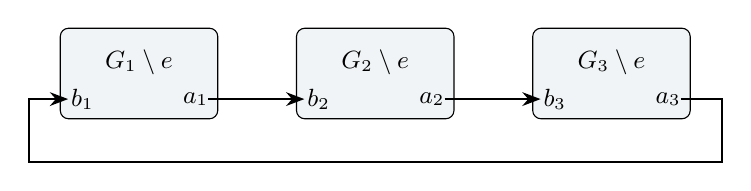
\begin{tikzpicture}[>=Stealth,font=\small]
\foreach \x/\n in {0/1,3/2,6/3}{
 \draw[rounded corners=3pt,fill=Light] (\x,0) rectangle +(2,1.15);
 \node at (\x+1,0.72) {$G_{\n}\setminus e$};
 \node at (\x+0.28,0.25) {$b_{\n}$};
 \node at (\x+1.72,0.25) {$a_{\n}$};
}
\draw[->,thick] (1.88,0.25)--(3.10,0.25);
\draw[->,thick] (4.88,0.25)--(6.10,0.25);
\draw[->,thick] (7.88,0.25) -- (8.4,0.25) -- (8.4,-0.55) -- (-0.4,-0.55)
 -- (-0.4,0.25) -- (0.1,0.25);
\end{tikzpicture}
\caption{Cyclic amplification for three copies. Each box is connected after
one non-bridge edge is removed. Reconnecting the exposed slots preserves
every color count. Arrows indicate the re-pairing prescription, not an
orientation on Wick edges.}
\label{wick:fig:rewire}
\end{figure}

\begin{theorem}[Equality of connected and full diagramwise domains]
\label[theorem]{wick:thm:connected}
Assume $\abs{\alpha^a}\ge2$ for every interaction type. The connected vacuum
Wick family is strongly summable if and only if the full vacuum family is
strongly summable. Equivalently, its exact domain is the finite cone of
\Cref{wick:thm:main}.

If the criterion fails, there is an indecomposable vector $h$ of nonpositive
weight and, for every $n\ge1$, a connected diagram with leading exponent
$nL(h)$. Thus the obstruction can be realized by connected diagrams of
arbitrarily large size.
\end{theorem}
\begin{proof}
The connected family is a subfamily of the full family, so full summability
implies connected summability. For the converse, if the full criterion
fails, \Cref{wick:cor:obstruction} gives an $h\in\cH$ with $L(h)\le0$. The
integer incidence equation guarantees that at least one pairing realizes
$h$, by \Cref{wick:lem:wickcount}. It is connected by
\Cref{wick:lem:indecompconnected}. Apply \Cref{wick:lem:rewire}. The amplitudes of the
resulting connected graphs are nonzero rational multiples of
$g^{nm}C^{nk}$, so they have leading exponents $nL(h)$. A negative weight
produces a descending support sequence; a zero weight produces infinitely
many terms with exponent zero. Either contradicts strong summability of the
connected family.
\end{proof}

\subsection{The connected logarithm on the admissible domain}

\begin{proposition}[Specialization of the connected identity]
\label[proposition]{wick:prop:connectedlog}
Under the equivalent conditions of \Cref{wick:thm:main}, write $Z=1+z$. Then
either $z=0$ or $\val(z)>0$. The Hahn series
\begin{equation}
 \log Z=\sum_{n\ge1}\frac{(-1)^{n+1}}{n}z^n
 \label{wick:eq:log}
\end{equation}
is defined and equals the strongly summed connected vacuum Wick family.
\end{proposition}
\begin{proof}
Every nonempty atom has positive valuation by the criterion. Their family
is strongly summable; its support union, when nonempty, is a well-ordered
subset of $\Gamma_{>0}$ and therefore has a positive minimum. Cancellation
can only raise the valuation of their sum. This proves the assertion about
$z$ and makes \eqref{wick:eq:log} valid by \Cref{wick:cor:substitution}.

For completeness, the classical combinatorial identity can be expressed
without graph symmetry conventions. Give the vertices of each interaction
type separate labels and distinguish their colored slots. Every pairing is
uniquely a set of connected pairings on a partition of these labeled
vertices. In the exponential generating function, the factors $1/m_a!$
remove the vertex labels; the factors $1/r!$ in an exponential remove the
ordering of the $r$ components. Consequently the formal sum of all pairings
is the exponential of the formal sum of connected pairings. This is an
identity in finitely many formal coupling and edge variables, with only
finitely many objects contributing to each coefficient. It is the usual
connected-diagram identity \cite[Section 3.5]{Etingof}.

Use the balancing vector to substitute the positive-valuation entries
$u_a,w_e$ of \eqref{wick:eq:scaleddata}. \Cref{wick:cor:substitution} respects the
formal identity, and the vacuum scaling factors cancel. Taking the formal
logarithm, evaluated by \eqref{wick:eq:log}, gives the claimed equality.
\end{proof}

\begin{example}[Why linear vertices are different]
\label[example]{wick:ex:linear}
For one variable, $P=gx$ and covariance $C=c\ne0$, the full vacuum family is
\[
 Z=\sum_{n\ge0}\frac{(g^2c/2)^n}{n!}.
\]
It is strongly summable exactly when $\val(g^2c)>0$. But the connected
vacuum family has only the single two-vertex graph and sums to $g^2c/2$
for every $g,c$. A graph with all vertices of valence one is a disjoint
union of isolated edges, so it has no non-bridge edge to amplify. This shows
that the valence hypothesis in \Cref{wick:thm:connected} cannot simply be deleted.
Outside the full domain, the finite connected sum is not being asserted to
be the Hahn logarithm of a nonexistent vacuum sum.
\end{example}

\section{Positive covariance and sharp stationary-phase scaling}
\label{wick:sec:positive}

\subsection{A collapse to one inequality per monomial}

A real symmetric matrix $C$ over $\KR$ is positive definite if
$x^TCx>0$ for every nonzero $x\in\KR^d$. This is an ordered-field condition.
It is not the statement that every coefficient of every entry is positive.

\begin{lemma}[Valuation Cauchy--Schwarz]
\label[lemma]{wick:lem:valCS}
If $C$ is positive definite, then $C_{ii}>0$ and, for every nonzero
$C_{ij}$,
\begin{equation}
 c_{ij}\ge\frac{c_{ii}+c_{jj}}2.
 \label{wick:eq:valCS}
\end{equation}
\end{lemma}
\begin{proof}
Positivity on a coordinate vector gives $C_{ii}>0$. For $i\ne j$, apply
positivity to the vector with coordinates $-C_{ij}$ at $i$ and $C_{ii}$
at $j$. Its quadratic value is
$C_{ii}(C_{ii}C_{jj}-C_{ij}^2)>0$, hence
$C_{ii}C_{jj}>C_{ij}^2$. If $2c_{ij}<c_{ii}+c_{jj}$, the negative term
$-C_{ij}^2$ would be the leading term of their difference and would make
that difference negative. This is impossible. The diagonal case is equality.
\end{proof}

\begin{theorem}[Positive-covariance criterion]
\label[theorem]{wick:thm:positive}
For positive-definite $C$ over $\KR$, define
\begin{equation}
 \delta_a=\lambda_a+\frac12\sum_i\alpha_i^a c_{ii}.
 \label{wick:eq:delta}
\end{equation}
The full Wick family is strongly summable if and only if
\begin{equation}
 \delta_a>0\qquad(1\le a\le s).
 \label{wick:eq:deltacriterion}
\end{equation}
The same equivalence holds for an arbitrary diagonal covariance matrix over
$\K$ with all diagonal entries nonzero, without a positivity assumption.
For positive-definite $C$, an explicit balancing vector is
\begin{equation}
 p_i=\frac{c_{ii}}2-\varepsilon,
 \quad 0<\varepsilon<\min_a\frac{\delta_a}{\abs{\alpha^a}},
 \label{wick:eq:explicitpositivebalance}
\end{equation}
whenever \eqref{wick:eq:deltacriterion} holds.
\end{theorem}
\begin{proof}
For necessity, fix $a$ and take $m=2\ve_a$. Pair all slots using diagonal
edges: set $k_{ii}=\alpha_i^a$ and every cross-edge count to zero. This is a
nonzero member of $S$ with weight $2\delta_a$. \Cref{wick:thm:main} requires that
weight to be positive.

For sufficiency, take any $(m,k)\in S$. By \Cref{wick:lem:valCS},
\begin{align*}
 \sum_{i\le j}k_{ij}c_{ij}
 &\ge\frac12\sum_i c_{ii}(Dk)_i
 =\frac12\sum_i c_{ii}(Am)_i,\\
 L(m,k)&\ge\sum_a m_a\delta_a.
\end{align*}
A nonzero element of $S$ has $m\ne0$, because $Dk=0$ with $k\ge0$ forces
$k=0$. The last expression is therefore strictly positive if all $\delta_a$
are positive. Apply \Cref{wick:thm:main}.

For diagonal covariance, the first inequality is an equality. The same
necessity and sufficiency arguments thus apply without ordering its entries.
Finally, \eqref{wick:eq:explicitpositivebalance} gives
\[
 \lambda_a+\alpha^a\cdot p
 =\delta_a-\abs{\alpha^a}\varepsilon>0,
\]
and, by \eqref{wick:eq:valCS},
\[
 c_{ij}-p_i-p_j
 =c_{ij}-\frac{c_{ii}+c_{jj}}2+2\varepsilon\ge2\varepsilon>0.
\]
A suitable $\varepsilon$ exists by taking half the finite positive minimum
in \eqref{wick:eq:explicitpositivebalance}.
\end{proof}

The theorem concerns a real positive covariance but permits complex
couplings. Its diagramwise criterion is insensitive to their phases.
Complex phases can nevertheless cause cancellations after grouping; the
example in \Cref{wick:sec:cancellation} uses $C=I$ and does not contradict this
theorem because it asks for a different kind of sum.

\subsection{An algebraic stationary-phase domain}

Consider the polynomial action
\begin{equation}
 \mathcal S(x)=\frac12\sum_{i=1}^d q_i x_i^2
                 +\sum_{a=1}^s u_a x^{\alpha^a},
 \qquad q_i,u_a,\hbar\in\K^\times,
 \quad\abs{\alpha^a}\ge3.
 \label{wick:eq:action}
\end{equation}
Its normalized perturbative Gaussian expression has diagonal covariance
$C_{ii}=\hbar/q_i$ and couplings $g_a=-u_a/\hbar$. This is a definition by
Wick expansion, not an assertion that an integral over a surcomplex domain
has been constructed. It isolates the perturbative part, without an
additional Gaussian determinant prefactor.

\begin{corollary}[Sharp multiscale power counting]
\label[corollary]{wick:cor:stationary}
Set $h=\val(\hbar)$, $a_i=\val(q_i)$, and $b_a=\val(u_a)$. The normalized
Wick expansion for \eqref{wick:eq:action} is diagramwise strongly summable
exactly when
\begin{equation}
 \Delta_a=b_a+
 \left(\frac{\abs{\alpha^a}}2-1\right)h
 -\frac12\sum_i\alpha_i^a a_i>0
 \qquad\text{for every }a.
 \label{wick:eq:stationarycone}
\end{equation}
The same criterion governs every pairable monomial insertion and the
connected vacuum expansion. Every polynomial insertion is then defined by
the finite linear combination of its monomial sectors; cancellation between
those sectors is not needed for the criterion.
\end{corollary}
\begin{proof}
Substitute $\lambda_a=b_a-h$ and $c_{ii}=h-a_i$ into
\eqref{wick:eq:delta}. This gives $\delta_a=\Delta_a$. The diagonal part of
\Cref{wick:thm:positive} proves the exact criterion, \Cref{wick:thm:main} gives the
observable statement, and \Cref{wick:thm:connected} applies because all valences
are at least three.
\end{proof}

When the Hessian and interaction coefficients have valuation zero and
$h>0$, the inequalities are automatic for degrees at least three. This is
the familiar degree counting behind a formal stationary-phase expansion,
not a new discovery; compare \cite[Chapters 2--3]{Etingof}. The extra content
of \eqref{wick:eq:stationarycone} is its exact necessity and sufficiency when the
Hessian and couplings themselves occupy different, possibly non-Archimedean,
scales.

For one quartic term, the condition becomes
\begin{equation}
 b+h-2a>0.
 \label{wick:eq:quarticthreshold}
\end{equation}
At equality, infinitely many nonzero diagram atoms have the same leading
exponent. Below it, those exponents descend. Thus the strict boundary cannot
be repaired by replacing $>$ with $\ge$. A change in the valuation of a
degenerating quadratic coefficient can move an otherwise admissible
perturbative model across this boundary.

\section{Observables, exact identities, and truncation}
\label{wick:sec:observables}

\subsection{Normalized polynomial expectations}

Assume henceforth that the main criterion holds. For
$f=\sum_\beta f_\beta x^\beta\in\K[x_1,\ldots,x_d]$, define
\[
 \cZ_f=\sum_\beta f_\beta\cZ_\beta,
 \qquad \langle f\rangle_P=Z^{-1}\cZ_f.
\]
These are finite sums of well-defined Hahn values. The inverse of $Z=1+z$
is given by the strongly summable geometric series
$\sum_{n\ge0}(-z)^n$. In particular, $Z$ is never zero on the diagramwise
admissible domain. The construction is linear in $f$ and normalized by
$\langle1\rangle_P=1$.

\begin{lemma}[Algebraic Gaussian integration by parts]
\label[lemma]{wick:lem:ibp}
For every polynomial $f$,
\begin{equation}
 \EE_C[x_i f]=\sum_j C_{ij}\EE_C[\partial_j f].
 \label{wick:eq:ibp}
\end{equation}
\end{lemma}
\begin{proof}
It suffices to take $f=x^\beta$. In each pairing of the slots of
$x_i x^\beta$, the distinguished additional $i$-slot is paired with one of
the $\beta_j$ slots of color $j$. Removing that pair leaves a pairing of the
slots of $x^{\beta-\ve_j}$ and contributes the factor $C_{ij}$. Summing over
its possible partners gives
$\sum_{j:\beta_j>0}\beta_j C_{ij}\EE_C[x^{\beta-\ve_j}]$, which is the
right-hand side. Restricting to $\beta_j>0$ avoids negative monomial
exponents; the omitted polynomial derivatives are zero.
\end{proof}

\begin{theorem}[Exact perturbative Schwinger--Dyson identities]
\label[theorem]{wick:thm:SD}
For every polynomial $f$ and every $i$,
\begin{equation}
 \boxed{\quad
 \langle x_i f\rangle_P
 =\sum_j C_{ij}\bigl\langle\partial_j f+f\,\partial_j P\bigr\rangle_P.
 \quad}
 \label{wick:eq:SD}
\end{equation}
No invertibility assumption on $C$ is needed.
\end{theorem}
\begin{proof}
First treat the coefficients of $P$ as independent formal coupling
variables. Apply \eqref{wick:eq:ibp} to each polynomial coefficient of
$f\exp(P)$ in those variables. Formal differentiation gives
\[
 \partial_j(f\exp(P))=(\partial_j f+f\partial_jP)\exp(P).
\]
This yields the unnormalized version of \eqref{wick:eq:SD} coefficientwise.
Every fixed coefficient involves a polynomial and finitely many pairings.

To justify the specialization, use a balancing vector. Each observable
family is the evaluation of a formal power series in the finitely many
positive-valuation entries $u_a,w_e$, multiplied by one fixed monomial as
in \eqref{wick:eq:scaledatom}. The extra polynomial derivatives introduce only
finitely many observable families and fixed Hahn factors. Thus all formal
reindexings in the identity are legitimate strong sums. Evaluation gives
the unnormalized equality in $\K$. Multiply by $Z^{-1}$.
\end{proof}

Here $\partial_j$ means ordinary formal differentiation in the polynomial
variable $x_j$. It is not the Berarducci--Mantova derivation on surreal
scalars and not an all-scale analytic derivative. The theorem asserts a
Hahn-valued algebraic identity, not an integration theorem for a measure.

Formal coupling differentiation similarly gives
\[
 \frac{\partial Z}{\partial g_a}=\cZ_{\alpha^a},\qquad
 \frac{\partial\log Z}{\partial g_a}=\langle x^{\alpha^a}\rangle_P.
\]
These equations are first identities in independent formal coupling
variables. Their differentiated series may then be specialized on the
admissible domain, by the observable theorem. They do not endow all of
$\SC$ with a new scalar derivation.

\subsection{Support-aware truncation bounds}

For a fixed $\beta$, let $\cZ_{\beta,\le N}$ be the sum over the finitely
many atoms with $\abs m\le N$. Finiteness follows because $m$ has finitely
many possibilities and each determines a fixed finite number of slots.
Although each individual atom may have infinite Hahn support, this is a
finite algebraic expression in the input entries.

\begin{proposition}[A valuation error estimate]
\label[proposition]{wick:prop:tail}
Choose a balancing vector $p$ and a positive $\eta\in\Gamma$ no greater
than the valuations of all scaled entries $u_a,w_e$. Then
\begin{equation}
 \val\bigl(\cZ_\beta-\cZ_{\beta,\le N}\bigr)
 \ge p\cdot\beta+(N+1)\eta.
 \label{wick:eq:tail}
\end{equation}
The convention is that a zero tail has valuation $+\infty$.
\end{proposition}
\begin{proof}
An atom in the tail has $\abs m\ge N+1$. In the scaled expression
\eqref{wick:eq:scaledatom}, its valuation is at least
$p\cdot\beta+(\abs m+\abs k)\eta$, hence at least the right-hand side of
\eqref{wick:eq:tail}. Every exponent of the atom is at least its leading exponent.
The entire tail is a subfamily of a strongly summable family, and adding its
coefficients cannot create an exponent below this common bound.
\end{proof}

The estimate is useful but must not be overinterpreted. In a higher-rank
group, the sequence $n\eta$ may be bounded above by a much larger positive
element. Thus \eqref{wick:eq:tail} does not generally imply convergence of the
partial sums in the intrinsic valuation topology. Strong summability and
topological convergence are separate statements.

\begin{example}[An exact sum with nonconvergent truncations]
\label[example]{wick:ex:ranktwo}
Take $\Gamma=\Q^2$ with lexicographic order, one variable, $C=1$, and
$P=t^{(0,1)}x^4$. The vacuum sum is
\[
 Z=\sum_{n\ge0}\frac{(4n-1)!!}{n!}\,t^{(0,n)}.
\]
Its support is well ordered, with one nonzero term at each indicated
exponent, so it is a Hahn series. The tail after order $N$ has valuation
$(0,N+1)$, which is always less than $(1,0)$. It never enters the valuation
neighborhood requiring error valuation greater than $(1,0)$. The
truncations therefore do not converge to $Z$ in that topology.

Under the explicit embedding in \Cref{wick:prop:embedding}, these scales become
$\omega^{-n}$ and $\omega^{-\omega}$, respectively. The sum is exact as a
surreal normal form even though finite truncation does not approximate it
at the latter scale.
\end{example}

\section{Explicit models and sharp boundaries}
\label{wick:sec:examples}

\subsection{A divergent complex series with an exact surreal value}

Let $C=1$ and $P=-g x^4$. There is one atom per interaction order, and
\begin{equation}
 Z(g)=\sum_{n\ge0}(-1)^n\frac{(4n-1)!!}{n!}g^n
 =1-3g+\frac{105}{2}g^2-\frac{3465}{2}g^3+\cdots.
 \label{wick:eq:quartic}
\end{equation}
The convention is $(-1)!!=1$. If $a_n$ denotes the coefficient of $g^n$,
then
\[
 \frac{a_{n+1}}{a_n}
 =-\frac{(4n+1)(4n+3)}{n+1}.
\]
Its absolute value tends to infinity, so the ordinary complex power series
has radius of convergence zero. Nevertheless, \Cref{wick:thm:positive} says that
\eqref{wick:eq:quartic} has a strong Hahn value for every $g$ with $\val(g)>0$.
For $g=t$ and $t\mapsto\omega^{-1}$ this gives the explicit surreal number
\[
 1-3\omega^{-1}+\frac{105}{2}\omega^{-2}
 -\frac{3465}{2}\omega^{-3}+\cdots.
\]
The result is a normal-form value, not an assertion that it equals the
integral of a Gaussian function over a surreal line.

The connected logarithm begins
\begin{equation}
 \log Z(g)=-3g+48g^2-1584g^3+\cdots.
 \label{wick:eq:quarticlog}
\end{equation}
The accompanying program obtains $3$, $48$, and $1584$ independently by
enumerating the connected labeled pairings at orders one, two, and three,
and compares them with the formal logarithm coefficients. The ordinary
combinatorial coefficients are classical; their exact specialization domain
is the point of the example.

\subsection{An infinite coupling can be admissible}
\label{wick:sec:cubic}

Take two variables and the purely cross covariance
\[
 C=\begin{pmatrix}0&c\\c&0\end{pmatrix},\qquad c\ne0,
 \qquad P=gx^3+hy^3.
\]
A vacuum pairing requires $3m_1=k_{12}=3m_2$, so
\[
 S=\N(1,1;3).
\]
There is just one Hilbert generator, and the criterion is
\begin{equation}
 \val(g)+\val(h)+3\val(c)>0.
 \label{wick:eq:cubiccriterion}
\end{equation}
The exact sum is
\begin{equation}
 Z=\sum_{n\ge0}\frac{(3n)!}{(n!)^2}(ghc^3)^n.
 \label{wick:eq:cubicZ}
\end{equation}
The coefficient counts all bijections between the $3n$ slots of each color.

For $g=t^{-100}$, $h=t^{101}$, and $c=1$, condition
\eqref{wick:eq:cubiccriterion} is satisfied. One coupling is infinite, yet each
realizable vacuum product has increasing valuation. The exact solver
returns, for instance,
\[
 p_x=\frac{67}{2},\qquad p_y=-\frac{403}{12}.
\]
The three strict residuals are $1/2$, $1/4$, and $1/12$, respectively.
This explicitly demonstrates how an infinite coupling can be compensated
by covariance and incidence scaling.

If only the monomial $gx^3$ is present with the same purely cross covariance,
then $S=\{0\}$. Every nonempty vacuum moment vanishes because there are no
$y$-slots to pair with. Thus $Z=1$ for arbitrary nonzero $g$, in agreement
with the vacuous Hilbert-basis test. Adding $hy^3$ creates a genuine new
cycle condition; checking each interaction in isolation would miss it.

\subsection{A mixed quartic instability with a four-element Hilbert basis}
\label{wick:sec:mixed}

Let
\[
 P=g_1x^4+g_2y^4,
 \qquad C_{11},C_{12},C_{22}\ne0.
\]
Use the coordinate order $(m_1,m_2;k_{11},k_{12},k_{22})$. The incidence
relations are
\[
 4m_1=2k_{11}+k_{12},\qquad
 4m_2=2k_{22}+k_{12}.
\]
They imply $k_{12}=2s$ and
\[
 (m_1,m_2;k_{11},k_{12},k_{22})
 =(m_1,m_2;2m_1-s,2s,2m_2-s),
 \quad0\le s\le2\min(m_1,m_2).
\]

\begin{proposition}[Exact quartic Hilbert basis and irredundant tests]
\label[proposition]{wick:prop:quarticH}
The Hilbert basis consists of
\begin{align*}
 h_1&=(1,0;2,0,0),& h_2&=(0,1;0,0,2),\\
 h_3&=(1,1;1,2,1),& h_4&=(1,1;0,4,0).
\end{align*}
The summability criterion reduces to the three inequalities
\begin{align}
 w_1&=\lambda_1+2c_{11}>0,\nonumber\\
 w_2&=\lambda_2+2c_{22}>0,\label{wick:eq:quartictests}\\
 w_4&=\lambda_1+\lambda_2+4c_{12}>0.\nonumber
\end{align}
\end{proposition}
\begin{proof}
If $s=2r$, the count vector is
$r h_4+(m_1-r)h_1+(m_2-r)h_2$.
If $s=2r+1$, it is
$r h_4+h_3+(m_1-r-1)h_1+(m_2-r-1)h_2$.
The indicated coefficients are nonnegative by the bound on $s$. This
proves generation. Each of the four vectors is indecomposable: $h_1,h_2$
have one vertex, while any nontrivial split of $h_3$ or $h_4$ would have to
split their vertex vector $(1,1)$ into $(1,0)+(0,1)$, which permits only
diagonal pairings and cannot supply their positive cross-edge count.

The weight of $h_3$ is
\[
 w_3=\lambda_1+\lambda_2+c_{11}+2c_{12}+c_{22}
     =\frac{w_1+w_2+w_4}{2}.
\]
Thus its inequality follows from the other three. None of those three
follows from the other two: with $c_{11}=c_{22}=0$, one can make either
$\lambda_1$ or $\lambda_2$ negative and choose the other and $c_{12}$ large
enough; or take both $\lambda_i>0$ and choose $c_{12}$ sufficiently negative.
This proves the stated reduction and irredundancy.
\end{proof}

Now choose the monomial data
\begin{equation}
 C=\begin{pmatrix}t^2&1\\1&t^2\end{pmatrix},
 \qquad g_1=g_2=t^{-1}.
 \label{wick:eq:mixedmodel}
\end{equation}
Then $w_1=w_2=3>0$ and $w_3=2>0$, but $w_4=-2$. Each quartic interaction
by itself is admissible, while their combination is not. The offending
family with $m_1=m_2=n$ and all edges cross-colored has atoms
\begin{equation}
 \frac{(4n)!}{(n!)^2}\,t^{-2n}.
 \label{wick:eq:mixedbad}
\end{equation}
Their leading exponents form a strictly descending sequence. The solver returns precisely
$h_4=(1,1;0,4,0)$ as its primitive obstruction certificate. The two-vertex
four-edge realization is connected, and cyclic amplification gives
connected obstructing diagrams at every multiple size.

The matrix in \eqref{wick:eq:mixedmodel} is invertible, since its determinant is
$t^4-1\ne0$, but it is not positive definite. Thus this is a legitimate
surcomplex bilinear Gaussian model, and it cannot occur under the hypotheses
of \Cref{wick:thm:positive}. All its displayed coefficients are positive, so the
obstruction is not merely an artifact of a cancellation-sensitive
presentation: grouping by interaction order cannot erase it.

\subsection{A genuinely higher-rank boundary}
\label{wick:sub:rankboundary}

In the cross-cubic model, choose $\Gamma=\Q^2$ lexicographically. The entire
criterion is the sign of
\[
 w=\val(g)+\val(h)+3\val(c)\in\Q^2.
\]
A weight $(0,1)$ is admissible and $(0,-1)$ is not. Both have first coordinate
zero. A weight $(1,-10^6)$ is positive and admissible, despite its large
negative second coordinate. Replacing the value group by its first real
coordinate cannot decide the boundary.

For the inputs $\val(g)=(0,0)$, $\val(h)=(0,1)$, and $\val(c)=(0,0)$,
the solver returns
\[
 p_x=(0,1/6),\qquad p_y=(0,-1/4),
\]
with strictly positive residuals $(0,1/2)$, $(0,1/4)$, and $(0,1/12)$.
Changing $\val(h)$ to $(0,-1)$ instead produces the integer obstruction
$(1,1;3)$. The same finite incidence problem detects the second-scale
transition exactly.

\section{Cancellation, grouping, and the precise boundary of the theorem}
\label{wick:sec:cancellation}

\subsection{An isotropic counterexample to a stronger claim}

The criterion is not necessary for every imaginable way of first combining
diagrams. This is not a technical concern confined to exotic covariances.
Take the positive-definite real covariance $C=I_2$ and the complex linear
form $\ell=x+iy$. Its bilinear Wick covariance is
\[
 \EE_C[\ell^2]=1+i^2=0.
\]
By multilinearity of Wick pairings, for every $r\ge1$,
\begin{equation}
 \EE_C[\ell^{2r}]=(2r-1)!!\bigl(\EE_C[\ell^2]\bigr)^r=0.
 \label{wick:eq:isotropicmoments}
\end{equation}
Let
\begin{equation}
 P=t^{-1}(x+iy)^4.
 \label{wick:eq:isotropicP}
\end{equation}
After expanding into distinct monomials, every nonzero coupling has valuation
$-1$, while the diagonal covariance valuations are zero. The exact
positive-covariance criterion therefore fails for every interaction
monomial. In particular, the $t^{-1}x^4$ monomial alone contributes a
subfamily with strictly descending leading exponents.

But grouping the entire polynomial power $P^n$ \emph{before} summing over
$n$ gives
\begin{equation}
 \frac1{n!}\EE_C[P^n]=0\quad(n\ge1),\qquad
 Z_{\mathrm{grouped}}=1.
 \label{wick:eq:groupedone}
\end{equation}
Each cancellation in \eqref{wick:eq:groupedone} is finite, but there are
infinitely many such blocks. The raw family is illegal as a Hahn sum while
the block family is legal. Finite regrouping preserves an already strong
sum; it does not imply the reverse statement when cancellations remove
supports from infinitely many blocks.

This example also explains why the criterion is diagonal-monomial invariant
but not invariant under arbitrary complex linear changes of coordinates.
Using isotropic coordinates can encode a cancellation in the covariance
pattern itself. A coordinate-independent classification of all possible
cancellation-aware sums is a different problem.

\subsection{A class in which order grouping does not help}

A Hahn series is \emph{coefficientwise nonnegative} if every coefficient is
a nonnegative real number. This is stronger than being positive in the
ordered field, which requires only a positive leading coefficient.

\begin{proposition}[Sign-coherent equivalence]
\label[proposition]{wick:prop:signcoherent}
Suppose every nonzero covariance entry is coefficientwise nonnegative, and
$g_a=\sigma u_a$ for a common $\sigma\in\C^\times$, where each $u_a$ is a
nonzero coefficientwise nonnegative Hahn series. Then the following are
equivalent:
\begin{enumerate}[label=\textup{(\roman*)}]
\item the raw Wick atom family in a fixed sector $Q_\beta$ is strongly summable;
\item the family obtained by grouping all atoms with the same total
interaction order $\abs m=n$ is strongly summable.
\end{enumerate}
For a pairable sector, both are equivalent to \Cref{wick:thm:main}.
\end{proposition}
\begin{proof}
At order $n$, every atom is $\sigma^n$ times a nonzero coefficientwise
nonnegative Hahn series. Its coefficient multiplier in \eqref{wick:eq:atom} is
positive rational. After factoring out the same nonzero complex number
$\sigma^n$, no coefficient cancels within an order block,
and the support of the block is exactly the union of the supports of its
atoms. Each block contains finitely many atoms.

If the block family is strongly summable, its support union is well ordered
and any fixed exponent occurs in only finitely many blocks. Since every
block is finite and no support is erased, the exponent occurs in only
finitely many raw atoms. This proves raw strong summability. The other
implication is the ordinary regrouping property of strong sums. The last
claim follows from \Cref{wick:thm:main}.
\end{proof}

The proposition includes the common-sign choices $\sigma=\pm1$ and permits
any common nonzero complex factor. It is a sufficient support-preservation
hypothesis, not a necessary classification of cancellation-free data.

The mixed obstruction \eqref{wick:eq:mixedmodel} satisfies this hypothesis.
For the quartic model \eqref{wick:eq:quartic}, there is already exactly one
atom at each interaction order, so raw and order-grouped summability agree
for every nonzero Hahn coupling $g$, even when its coefficients have mixed
signs or phases. For example, $g=t-t^2$ has positive valuation but does not
become coefficientwise nonnegative after multiplication by any fixed
nonzero complex constant. The quartic domain is still exactly $\val(g)>0$.
The isotropic example, by contrast, erases supports within its order blocks
and shows why the reverse regrouping implication needs a hypothesis.

\section{Exact certificate computation and reproducible checks}
\label{wick:sec:code}

\subsection{What the implementation does}
\label{wick:sub:implementation}

A Python implementation using only the standard library is included in
this report's directory as \texttt{code/wick\_certificates.py}. Its
implemented value groups are $\Q^r$ with lexicographic order, for any
specified finite $r\ge1$.
A value is represented by a tuple of exact \texttt{Fraction} objects.
The routine forms the rows $A^T$ and $-D^T$, applies the strict elimination
algorithm of \Cref{wick:thm:alternative}, and returns one of two certificates:
a balancing vector $p$, or a primitive nonnegative integer obstruction
$(m,k)$. Every returned certificate is rechecked against the original
system using exact arithmetic.

For example, with the directory \texttt{code} on the Python import path,
the mixed-quartic obstruction can be reproduced by
\begin{lstlisting}[language=Python]
from wick_certificates import value, wick_certificate

certificate = wick_certificate(
    alphas=[(4, 0), (0, 4)],
    edges=[(0, 0), (0, 1), (1, 1)],
    coupling_values=[value([-1]), value([-1])],
    covariance_values=[value([2]), value([0]), value([2])],
)
assert certificate.obstruction == (1, 1, 0, 4, 0)
\end{lstlisting}
The code uses zero-based edge indices, while the mathematical notation uses
one-based variable indices. All listed covariance entries are assumed
nonzero; omitting an edge is how one specifies a zero entry. The code does
not inspect symbolic Hahn series to discover their valuations.

The implementation does not enumerate a general Hilbert basis. It bypasses
that potentially expensive task by using the equivalent balancing problem.
It also does not construct an arbitrary Hahn field, decide equality of
arbitrary surreal expressions, sum an analytic integral, or implement
arbitrary-rank ordered groups. Those would be different computational
capabilities. The mathematical theorem allows arbitrary rank; the supplied
executable tests use exact finite-rank representations.

\subsection{From a failed certificate to connected graphs}

There is a finite, though potentially expensive, way to refine an arbitrary
integer obstruction $q$ into the indecomposable obstruction used in
\Cref{wick:thm:connected}. Search the finite box $0\le q'\le q$ for a nonzero
proper solution of the same homogeneous incidence equations. If no such
$q'$ exists, $q$ is indecomposable. Otherwise
$q=q'+(q-q')$, and at least one summand has nonpositive weight. Replace $q$
by that summand and repeat. The sum of the coordinates decreases strictly,
so this terminates.

A pairing with the resulting counts can be built by allocating slots
according to the integer edge counts, as in the proof of
\Cref{wick:lem:wickcount}. It is connected automatically. Select a non-bridge
edge by checking connectivity after edge removal, and apply the cyclic
construction. Thus the obstruction theorem supplies an actual finite recipe
for connected counterexamples, not just an existence argument involving a
limit or an uncomputable search over all graphs. The supplied program tests
the cyclic construction on three types of base multigraph; it does not
implement this whole refinement pipeline for arbitrary inputs.

\subsection{The recorded test run}
\label{wick:sub:testrun}

Run the checks from the root of a \emph{copy} of this report's directory with
\begin{lstlisting}
python3 code/verify.py
\end{lstlisting}
The script writes \texttt{data/verification.json}. The random test seed is
\texttt{20260922}; no floating-point arithmetic is used in the mathematical
checks. The only floating-point quantity in the report is elapsed wall-clock
time. One counted case is one call to the script's explicit test-case
checker; additional internal assertions verifying every returned
certificate are not included in the count.

The output path is fixed relative to the script, not to the working
directory, and the file records the elapsed time. Every run therefore
rewrites the delivered record, which is why the command above is meant for a
copy. The internal certificate rechecks are \texttt{assert} statements, so
the script must not be run under Python's \texttt{-O} flag. The file
\texttt{code/Makefile} holds optional targets whose paths are relative to the
report root; from the root of a copy, \texttt{make -f code/Makefile check}
runs the suite and \texttt{make -f code/Makefile pdf} builds the article.
When this report was placed in the collection, the suite was rerun on a copy
under Python~3.14.4. It passed all 7,684 cases, and the rewritten record
agreed with the delivered one in every entry except the elapsed time.

\begin{table}[ht]
\centering\small
\begin{tabularx}{\textwidth}{Y r}
\toprule
Finite test family & Cases\\
\midrule
Two-quartic semigroup decomposition formula, $0\le m_1,m_2\le20$ & 6,181\\
Two-quartic feasibility versus its three closed-form inequalities & 540\\
Cross-cubic feasibility versus its single exact inequality & 300\\
Three-variable diagonal feasibility versus the monomial inequalities & 210\\
Vacuous vacuum-semigroup feasibility & 75\\
Colored Wick formula versus an independent moment recurrence & 300\\
Quartic total pairing counts & 3\\
Connected pairing counts versus formal logarithm coefficients & 3\\
Cyclic connected rewiring, including loops and parallel edges & 60\\
Exact isotropic cancellation identities & 12\\
\midrule
\textbf{Total passing cases} & \textbf{7,684}\\
\bottomrule
\end{tabularx}
\caption{The recorded finite checks. They test formulas and implementation
behavior; the infinite and arbitrary-rank statements are established by
the mathematical proofs, not by this table.}
\label{wick:tab:checks}
\end{table}

The feasibility checks include ranks one, two, and three. The moment check
uses an independent recurrence obtained by choosing the partner of the first
slot, rather than reusing the closed factorial formula. The connected check
enumerates all pairings of up to twelve labeled quartic half-edges and tests
graph connectivity directly. The cancellation check computes with integers
and powers of $i$, simplified exactly; it is not a numerical near-zero test.

A failed resource guard is reported as an exception. It is not reported as
infeasibility, and it does not constitute a mathematical counterexample.
This distinction is part of the solver's contract. Concretely, the guard is
the \texttt{max\_rows} argument of the solver, by default $200{,}000$
generated rows, and exceeding it raises \texttt{RuntimeError}. Fourier--Motzkin
elimination can need exponentially many rows, so on large inputs the guard,
not the mathematics, may decide whether an answer is returned at all.

\section{Novelty audit, sources, and limitations}
\label{wick:sec:provenance}

\subsection{Repository scope}
\label{wick:sub:reposcope}

The repository inspection was pinned to the main-tree commit
\begin{center}\small\Commit\end{center}
so that its conclusions do not depend on a moving branch. The inspected
\texttt{docs/README.md} catalogs 26 reports in five families and emphasizes
that the research drafts, finite verification programs, and Lean coverage
are different kinds of evidence \cite{Repo}. The catalog includes Hahn
analysis, finite deformations, polynomial algebra, spectral theory, dynamics,
physics, and several other surreal topics. No report in that catalog is
identified as a finite-certificate Wick summability theory.

The opening 190 lines of the physics report were also inspected. They
concern the scope of replacing real and complex scalars in physics,
including singular spacetime calculations and distinctions between symbolic
and physical conclusions. The present work instead fixes a finite algebraic
Gaussian model and determines its exact support domain. This is a different
question, not a proposed resolution of a spacetime singularity. The source
read no further into that report; its passages on perturbative families
bear directly on the present subject, and the relation is stated in
\Cref{wick:sub:physics}.

The recursive metadata for \texttt{docs/new} listed 18 ZIP archives,
including recent work on theta series, Tate uniformization, interpolation,
spectral theory, regular singular equations, holonomic rigidity, and
dynamics. Their filenames were inspected, but their internal texts were
\emph{not} exhaustively read. The repository connector rejected a binary
archive fetch, and attempted binary download and snapshot retrieval did not
succeed. The source manuscript reported that targeted repository searches
for \texttt{Wick} and \texttt{Gaussian}, made through the connector's code
search, returned no matches, and it treated these as negative search
observations that do not prove absence from compressed archives or
unindexed content.

\emph{Correction made when this report was placed in the collection.} For
\texttt{Gaussian} the reported result is not true of the tree at the pin. A
plain text search of the tree at that commit finds the word, in either
case, in twenty files; four of them are \texttt{article.tex} sources of reports. In the physics report it names
a Gaussian regulator: Computation~17.5 there, labelled
\texttt{phys:comp:gaussian}, whose two ordinary integrals show that an
unlimited value defines no product of distributions. Everywhere else it
means Gaussian-rational arithmetic (in the computer-algebra,
differential-equations, dynamics-and-normal-forms, spectral-theory and
infinite-dimensional spectral reports, mostly in their programs and data)
or Gaussian elimination (once, in the computer-algebra report). None of
these occurrences concerns a Gaussian perturbation expansion, a Wick
contraction or a diagram family, so the gap the source identified is real
even though its search result was not. For \texttt{Wick} the reported result
stands: the tree at the pin has no case-sensitive match, and its only
case-insensitive match is inside the German word \emph{Entwicklung}, in a
bibliography entry of the nonabelian-support report.

Accordingly, the accurate repository claim is: \emph{the theorem package was
not found in the repository materials successfully inspected}. A stronger
claim that every file and archive in the repository has been checked would
be unsupported. The accompanying \texttt{RESEARCH\_AUDIT.md} records paths,
searches, the snapshot identifier, and this access boundary. That file is
kept as delivered, so its sentence that both searches returned no matches
carries the correction above. The archives have since been opened; see
\Cref{wick:sub:collection}.

\subsection{Literature scope and what is not being claimed as new}

The following division of credit is part of the mathematical statement of
the project.

\begin{table}[ht]
\centering\small
\begin{tabularx}{\textwidth}{>{\raggedright\arraybackslash}p{0.33\textwidth}Y}
\toprule
Ingredient or result & Status in this manuscript\\
\midrule
Hahn supports and surreal normal forms & Classical foundations; use
\cite{Neumann,BM}.\\
Wick pairing coefficients and the connected logarithm & Classical formal
Gaussian combinatorics; compare \cite[Chapter 3]{Etingof}.\\
Dickson finiteness and strict elimination & Classical finite-dimensional
tools, reproved here; no priority claim.\\
Exact finite Hahn specialization cone & Proposed contribution in
\Cref{wick:thm:main}, with its observable and robustness conclusions.\\
Connected obstruction amplification & Proposed contribution in
\Cref{wick:thm:connected}; the valence boundary is explicit.\\
Positive-covariance collapse and multiscale thresholds & Consequences proved
in \Cref{wick:thm:positive,wick:cor:stationary}, presented as part of the theorem package.\\
Cancellation and sign-coherent boundary & Explicit limitations and exact
comparison results in \Cref{wick:sec:cancellation}.\\
\bottomrule
\end{tabularx}
\caption{Provenance of the mathematics. ``Proposed contribution'' means a
candidate novelty claim, not certified historical priority.}
\label{wick:tab:novelty}
\end{table}

Etingof's current author-hosted preliminary book was checked in addition to
the arXiv notes; its weighted Feynman theorem and connected-diagram theorem
are clear precedents for the formal combinatorics \cite{Etingof}. Neither
Wick's theorem nor formal stationary-phase degree counting is asserted to
originate here. Work on higher-rank Hahn geometry, such as
Joswig--Smith \cite{JoswigSmith}, is also relevant background, but the
present argument does not depend on an analytic convergence theorem for
multiple indeterminates.

Targeted web searches combining Hahn series, Wick expansions, Gaussian
perturbations, valuation balancing, and finite integer certificates did not
locate the precise results proved here. Some returned results were only
weakly relevant; this makes them particularly unsuitable as evidence of
absence. No exhaustive bibliographic search or expert priority review has
been completed. The conservative assessment is that the exact combination
of results is a plausible new contribution whose novelty remains to be
independently checked. This is distinct from uncertainty about what the
stated proofs assert: their hypotheses, deductions, and counterexamples are
all explicit and available for review.

\subsection{Mathematical boundaries}
\label{wick:sub:boundaries}

The model is finite-dimensional and has finitely many interaction monomials.
Its infinite aspect is the unbounded number of vertices and contractions,
not a continuum of field modes. There is no ultraviolet divergence,
renormalization construction, path measure, or nonperturbative completion
hidden in the notation. The finite criterion does not by itself extend to
an infinite list of couplings or covariance entries, where a union of
individually good support sets may fail to be well ordered or locally finite.

The theorem is about a prescribed monomial presentation and its Wick
pairings. It does not classify all cancellation-aware representations.
Strong summability is not ordinary analytic convergence, Borel summability,
or convergence of finite truncations in every higher-rank valuation
topology. A value in $\SC$ is supplied by an explicitly chosen normal-form
embedding, with set-sized supports; no unrestricted proper-class integral
or sum is introduced.

The exact verification program checks finite algebraic claims. It does not
verify the paper in Lean or another proof assistant. Current Lean coverage
is recorded separately in \texttt{docs/FORMALIZATION.md}:
\texttt{Surreal/Algebra/WickSemigroup.lean} proves Dickson finiteness,
the Hilbert-basis and observable-sector statements, and valuation
Cauchy--Schwarz; \texttt{Surreal/HahnSeries/NeumannWords.lean} proves
the positive-support lemma, including finite word multiplicity.
The strict alternative, full Wick summability equivalence, connected-domain
theorem and further specialization results are not yet formalized.
The build and axiom audit concern the imported declarations listed in that
ledger; finite test counts do not extend their proved scope.

\subsection{Relation to the physics report}
\label{wick:sub:physics}

The collection's physics report, \emph{Surreal Scalars in Theoretical
Physics} \cite{PhysReport}, sorts its own statements into exact symbolic
identities, conditional theorems proved in its text, and assessments, and it
does not let one kind be read as another. Nothing in the present report
belongs to that ledger. Its results are theorems about formal Gaussian
coefficient data over a Hahn field. They are not claims about physics, they
turn none of that report's assessments into a theorem, and none of that
report's statements is used here as a premise.

Three passages of that report touch the subject of this one. Section and
item numbers below are those of its build when this report was placed; at
that time it had not changed since the pin of \Cref{wick:sub:reposcope}.
\begin{enumerate}[label=\textup{(\alph*)}]
\item Its Section~17.2 (\texttt{phys:sub:formalpert}) is an assessment. It
displays a schematic triple-indexed transseries with algebraic, logarithmic
and exponentially small sectors, cautions that an arbitrary such family is
not automatically admissible, and adds that a Hahn or surreal realization
does not make an arbitrary formal expansion into a unique actual state or
scattering amplitude. Its non-claim N21 (Appendix~D.3) repeats the caution.
\item Its Computation~17.1 (\texttt{phys:comp:factorial}) is an exact
identity. The factorial series is a well-defined Hahn element at every
positive-valuation parameter, although the ordinary power series has zero
radius of convergence, and exact denotation does not give a real-valued sum.
\item Its Section~13.5 (\texttt{phys:sub:actions}) is an assessment. A
proper-class sum over surreal-valued histories is not licensed by Hahn
summability, and formal sums, finite-dimensional integrals and functional
measures are to be kept apart. Its non-claim N18 repeats the first part.
\end{enumerate}
The relation is the following, and no more.

The physics report poses no open problem on this subject, and this report
answers none of its questions. Passage~(a) says that admissibility is not
automatic. For one precisely delimited class of families, this report
decides it exactly. The class consists of the Wick diagram families of a
finite polynomial interaction with a symmetric bilinear covariance over
$\C((t^\Gamma))$, for divisible $\Gamma$: the vacuum family, every pairable
observable sector, and, when every valence is at least two, the connected
vacuum family. For these, \Cref{wick:thm:main,wick:thm:connected} reduce
strong summability to finitely many strict valuation inequalities. The
mixed quartic model of \Cref{wick:sec:mixed} is a family of this kind for
which strong summability fails although each of its two interactions alone
is admissible. This agrees with passage~(a) and gives it an exact form for
that class. It says nothing about the transseries display of passage~(a),
whose logarithmic and exponential sectors are not of Wick type, or about any
other family.

The quartic series \eqref{wick:eq:quartic} is the Wick counterpart of
passage~(b): an ordinary series of zero radius of convergence has an exact
Hahn value at every coupling of positive valuation. The physics report says
that exact denotation does not give a real-valued sum. This report says that
its value is a normal-form value, not the integral of a Gaussian function
over a surreal line (\Cref{wick:sec:examples}), and that it asserts no
solution to physical divergences (\Cref{wick:sec:conclusion}). The two
statements are consistent. Passage~(c) is respected throughout: every family
summed here is set-indexed in one set-sized Hahn workspace
(\Cref{wick:sec:hahn}), a Gaussian expectation is a finite sum over
pairings, and no path measure, functional integral or proper-class sum
occurs (\Cref{wick:sub:boundaries}). Finally, the isotropic example of
\Cref{wick:sec:cancellation} shows that even inside this class a grouped sum
can exist where the diagram family is not summable. Admissibility here is a
property of one prescribed family of terms, not of every way of assigning a
value to a formal expansion.

\subsection{This report in the collection}
\label{wick:sub:collection}

\emph{Provenance.} This report is built from a single manuscript,
\emph{Finite Certificates for Surcomplex Wick Summability}, dated 22 September
2026 and received as the archive \texttt{surcomplex\_wick\_certificates},
manuscript~12 of the eighteenth batch of external reports placed in the
collection. It is not a merge: there was no second source, and nothing was
selected out of a larger body of work. Every theorem, proof, example,
table and limitation originated in that manuscript; subsequent proof
corrections are recorded in the maintained README. Its repository audit is
pinned to \Commit. The delivered programs, recorded run and audit notes are
kept byte-identical: \texttt{code/wick\_certificates.py},
\texttt{code/verify.py}, \texttt{data/verification.json},
\texttt{VERIFICATION.md} and \texttt{RESEARCH\_AUDIT.md}, together with the
delivered \texttt{Makefile}, which was moved from the package root into
\texttt{code/}. The delivered README and PDF are not shipped. The PDF is
rebuilt from this source.

\emph{What changed on placement.} Every label now carries the prefix
\texttt{wick:}, and five subsections received labels they did not have. The
title page gained a status note and the abstract a sentence of scope.
\Cref{wick:sub:conventions}, \Cref{wick:sub:physics} and this subsection are
new, and the bibliography gained its entry for the physics report.
\Cref{wick:sub:implementation} now names this report's directory instead of
the delivered archive and says that \texttt{code} must be on the import
path. \Cref{wick:sub:testrun} gained the note on running the suite on a copy,
the location of the \texttt{Makefile}, the \texttt{-O} caveat (stated in the
delivered README and in \texttt{VERIFICATION.md}), the size of the resource guard and the record of
the rerun. \Cref{wick:sub:reposcope} gained the correction of the
\texttt{Gaussian} search result and pointers to the two new subsections.
Those placement changes did not alter mathematical statements or proofs.
The subsequent review recorded in the README is separate from placement.

\emph{Statements that were true at the pin and are now out of date.} At the
pin the catalogue \texttt{docs/README.md} listed 26 reports in five
families; the collection has grown since, and this report is one of the
additions. At the pin the 18 archives in \texttt{docs/new} could not be
opened by the source. They have since been unpacked and their manuscripts
placed in the collection's reports, and the directory \texttt{docs/new} no
longer exists. When this report was placed, their texts were searched: none
contains the word \texttt{Wick}, and \texttt{Gaussian} occurs in them only
as ``Gaussian rationals''. In the manuscripts placed with this one, the word
means Gaussian rationals, Gaussian elimination or Gaussian quadrature. When
this report was placed, no other report in the tree contained \texttt{Wick}
as a word or any of the terms Feynman, Schwinger, Hilbert basis or
Fourier--Motzkin. The source's provisional conclusion, that the theorem
package was not found in the repository materials inspected, therefore
extends to a text search of the whole tree at placement. It remains a text search, not a comparison of proofs, and
it says nothing about the published literature, where priority is still
unchecked (\Cref{wick:tab:novelty}).

\emph{Neighbouring reports.} The several-variable multiscale theta series
placed in the same batch in the report on Hahn--Tate uniformization is the
closest relative. Both characterize strong summability of a monomial family
indexed by an integer lattice or semigroup by a finite certificate, both
allow Hahn-unit tails and show that such tails cannot repair a failure, and
both assume divisible $\Gamma$. The mathematics differs: there a quadratic
energy on a lattice and its radical flags; here a linear weight on the
nonnegative integer kernel $S$, its Hilbert basis and the strict alternative
of \Cref{wick:thm:alternative}. Neither report uses a theorem of the other.
The distinction between strong summability and convergence of finite
subsums, illustrated here by \Cref{wick:ex:ranktwo}, is drawn throughout the
collection, beginning with its foundations report.

\section{Conclusions and further questions}
\label{wick:sec:conclusion}

The principal result is a complete support criterion for a large but
precisely bounded class of surcomplex expressions: finite polynomial
Gaussian perturbations with arbitrary symmetric Hahn covariance. Infinite
diagram summability is equivalent to a finite strict rescaling problem.
Its dual is an integer diagram pattern whose repetitions explain exactly
why summability fails. This interpretation survives arbitrary-rank value
groups and arbitrary higher Hahn coefficients.

Two refinements give the criterion more than a formal-substitution flavor.
The connected sector has the same obstruction domain once linear vertices
are excluded, because a non-bridge edge can amplify an indecomposable bad
pattern into connected patterns of every size. Positive real covariance,
on the other hand, prevents mixed contraction gains and reduces the full
cone to one inequality per interaction. These refinements explain both a
usable simplification and an explicit mechanism of failure.

The resulting values deserve to be called surcomplex when interpreted
through \Cref{wick:prop:embedding}: they are actual normal-form numbers, not
merely names for unperformed sums. Their interpretation is deliberately
algebraic. The quartic example becomes an exact surreal number despite
zero complex convergence radius; this says something definite about Hahn
support arithmetic without asserting a new measure theory or a solution to
physical divergences.

Three natural follow-on questions are newly posed here rather than claimed
to be established open problems in the literature. First, can the
cancellation-aware domain be described effectively for interactions with
specified algebraic symmetries, extending the isotropic example? Second,
which additional global support hypotheses permit countably many interaction
types while retaining a finite or finitely approximable certificate?
Third, for more restrictive graph families such as one-particle-irreducible
vacuum graphs, which obstruction patterns admit an amplification preserving
that stronger connectivity property? The present proofs identify precisely
where each extension would need new input.

\appendix
\section{Certificate verification without trusting the solver}
\label{wick:app:certificate}

A user of the algorithm can ignore its elimination trace and verify the
output directly. For a proposed balancing vector $p$, evaluate the finitely
many quantities
\[
 \lambda_a+\alpha^a\cdot p,\qquad c_{ij}-p_i-p_j.
\]
Every one must be strictly positive in the specified value-group order.
This proves summability by \Cref{wick:thm:main}.

For a proposed obstruction $(m,k)$, verify that its coordinates are
nonnegative integers, that it is not the zero vector, and that
\[
 Am=Dk,\qquad \lambda\cdot m+c\cdot k\le0.
\]
These tests prove failure of diagramwise summability without any appeal to
the solver. For example, the mixed-quartic witness
$(1,1;0,4,0)$ has
\[
 A(1,1)^T=(4,4)^T=D(0,4,0)^T,
 \qquad L=-1-1+4\cdot0=-2.
\]
The cross-cubic positive example has residuals
\begin{align*}
 -100+3\left(\frac{67}{2}\right)&=\frac12,\\
 101+3\left(-\frac{403}{12}\right)&=\frac14,\\
 0-\frac{67}{2}+\frac{403}{12}&=\frac1{12}.
\end{align*}
All these calculations are rational equalities. In rank two or higher,
each equality is evaluated componentwise and positivity is tested
lexicographically, using the first nonzero coordinate.

\section{A dependency map for the proofs}
\label{wick:app:dependencies}

The logical structure can be read without the examples or code. The
classical support lemma yields infinitesimal substitution. Integer color
balance and the explicit pairing count identify the exact leading
valuation of every atom. Dickson's lemma supplies a finite Hilbert basis.
The strict alternative equates positivity on its integer semigroup with
valuation balancing. Necessity follows by repeating one bad pattern;
sufficiency follows by balancing and infinitesimal substitution. These are
the two directions of \Cref{wick:thm:main}.

Connected-domain equality additionally uses only the finite-graph facts
that an indecomposable count vector has connected realizations and that a
connected multigraph of minimum valence two contains a non-bridge edge.
The positive-covariance theorem additionally uses only the ordered-field
$2\times2$ positivity inequality. The Schwinger--Dyson identity uses the
finite Wick recurrence, followed by the already justified substitution.
The counterexample to arbitrary grouping uses the exact algebraic identity
$1+i^2=0$.

Thus neither a numerical experiment, an analytic integral, nor an assumed
convergence theorem for infinite-rank topologies is a hidden premise of the
main proofs. The only imported infinitary algebraic input is the standard
Hahn support lemma; the surreal interpretation additionally uses the
standard normal-form laws.

\clearpage
\phantomsection\addcontentsline{toc}{section}{References}
\begin{thebibliography}{99}

\bibitem{Neumann}
B. H. Neumann,
\emph{On ordered division rings},
Transactions of the American Mathematical Society \textbf{66} (1949),
202--252.
\href{https://doi.org/10.1090/S0002-9947-1949-0032593-5}
{doi:10.1090/S0002-9947-1949-0032593-5}.

\bibitem{BM}
A. Berarducci and V. Mantova,
\emph{Surreal numbers, derivations and transseries},
Journal of the European Mathematical Society \textbf{20} (2018), 339--390.
\href{https://doi.org/10.4171/JEMS/769}{doi:10.4171/JEMS/769}.
Preprint: \href{https://arxiv.org/abs/1503.00315v3}{arXiv:1503.00315v3},
30 July 2015. See Section~2.3 for the Hahn-field identification,
Definition~2.9 and Remark~2.11 for summability, and Fact~2.17 for the
ordered-group omega-map used in the normal-form embedding.

\bibitem{Etingof}
P. Etingof,
\emph{Mathematical Ideas and Notions of Quantum Field Theory},
Graduate Studies in Mathematics, vol. 254,
American Mathematical Society, 2026.
Author-hosted preliminary version, 405 pages, inspected September 22, 2026:
\url{https://math.mit.edu/~etingof/gsm254.pdf}.
Related course notes:
\href{https://arxiv.org/abs/2409.03117v2}{arXiv:2409.03117v2},
revised August 28, 2026.
In the author-hosted book, see Sections 3.1--3.5, especially Theorems 3.8
and 3.11 (printed pages 37 and 41). The latter takes the logarithm of
the normalized partition function $Z/Z_0$; the present report's $Z$ is
already normalized. The book's printed page numbers and PDF page indices differ.

\bibitem{JoswigSmith}
M. Joswig and B. Smith,
\emph{Convergent Hahn series and tropical geometry of higher rank},
Journal of the London Mathematical Society \textbf{107} (2023), no. 4,
1450--1481.
\href{https://doi.org/10.1112/jlms.12716}{doi:10.1112/jlms.12716}.
Preprint: \href{https://arxiv.org/abs/1809.01457}{arXiv:1809.01457}.

\bibitem{Sauzin}
D. Sauzin,
\emph{Introduction to 1-summability and resurgence}, 2014.
\href{https://arxiv.org/abs/1405.0356}{arXiv:1405.0356}.
Used only to distinguish analytic Borel--Laplace summation from the
support-based summation considered here.

\bibitem{Repo}
V. Reshetnikov,
\emph{Surreal}, GitHub repository,
\url{https://github.com/VladimirReshetnikov/Surreal}.
Snapshot \Commit, inspected September 22, 2026.
Primary inspected text:
\href{https://github.com/VladimirReshetnikov/Surreal/blob/4cf691c7d951e037739d32d9f5c387dcce724f3c/docs/README.md}
{\texttt{docs/README.md}}.
Also inspected: the metadata tree for \texttt{docs/new}, and the beginning of
\texttt{docs/physics/surreal-scalars-and-spacetime/article.tex}.
Scope and access limitations are specified in \Cref{wick:sec:provenance}.

\bibitem{PhysReport}
\emph{Surreal Scalars in Theoretical Physics: Black-Hole Singularities,
Asymptotic Structure, and the Limits of Replacing the Scalar Field}.
Merged research report in the collection, directory
\nolinkurl{docs/physics/surreal-scalars-and-spacetime/}. Unchanged between the
snapshot of \cite{Repo} and the placement of this report. Only its
Sections~13.5 and~17.2--17.3 and its Appendix~D are referred to here, in
\Cref{wick:sub:physics}; none of its statements is used as a premise.

\end{thebibliography}
\end{document}
